\documentclass[english]{article}

% -----------------------------------------------------------------------------
% packages
% -----------------------------------------------------------------------------


% page and paragraph layout
% -------------------------
\usepackage[a4paper]{geometry}
\geometry{verbose,tmargin=1in,bmargin=1in,lmargin=1in,rmargin=1in}
%\setcounter{secnumdepth}{-2}
%\setcounter{tocdepth}{-2}
\usepackage{setspace}
\onehalfspacing%\doublespacing
\setlength{\parindent}{2.75em}
\setlength{\parskip}{1em}
\renewcommand{\baselinestretch}{1.5}
\usepackage{titlesec}
\titlespacing{\section}{0pt}{1.5ex}{-1.5ex}
\titlespacing{\subsection}{0pt}{1.5ex}{-1.5ex}
\titlespacing{\subsubsection}{0pt}{1.5ex}{-1.5ex}

% text style
% ----------
\usepackage{color}

% links
% -----
\usepackage{hyperref}

% paragraphs
% ----------
%\makeatletter
%\renewcommand{\@seccntformat}[1]{}
%\makeatother

% endnote
% -------
%\usepackage{endnotes}
%\let\footnote=\endnote
% bibliography
% ------------
%\usepackage[
%%natbib=true,
%backend=biber,
%%style=alphabetic,
%citestyle=authoryear,
%%hyperref=true,
%%maxbibnames=99,
%%firstinits=false
%%maxcitenames=4,
%%citetracker=true,
%%parentracker=true,
%bibstyle=authortitle,
%]{biblatex}


% exhibits
% --------
\usepackage{dcolumn}
\usepackage{tabularx,ragged2e}
\usepackage{threeparttable}
\usepackage{graphicx}
\usepackage{rotating}
%\usepackage[T1]{fontenc}
%\usepackage{times}
%\usepackage{amsmath}
%\usepackage{mathptmx}
%\usepackage{bbm}
%\usepackage{dsfont}
\usepackage{array,booktabs}
\usepackage{etoolbox}
\usepackage{caption}
\captionsetup[table]{labelfont=sc, labelsep=newline}
\renewcommand{\figurename}{Fig.}
\usepackage{etoolbox}
\usepackage{ctable}
\renewcommand{\thetable}{\Roman{table}}
\usepackage{csquotes}


% appendices
% ----------
\usepackage{appendix}


% tikz
% ----
% TO POPULATE


% -----------------------------------------------------------------------------
% load biblio
% -----------------------------------------------------------------------------
\bibliography{references.bib}

% -----------------------------------------------------------------------------
% cover page
% -----------------------------------------------------------------------------

\title{\LARGE Natural Experiments in Leadership Research:\\
       An Introduction, Review, and Guidelines}

\makeatletter
\renewcommand\@date{{%
    \begin{singlespace}
      \vspace{-\baselineskip}%
      \large\centering
      \begin{tabular}{@{}c@{}}
        Simone Santoni\textsuperscript{1} \\
        \normalsize \texttt{\href{simone.santoni.1@city.ac.uk}{simone.santoni.1@city.ac.uk}}
      \end{tabular}
      \quad \quad
      \begin{tabular}{@{}c@{}}
        Jost Sieweke\textsuperscript{2} \\
        \normalsize \texttt{\href{j.sieweke@vu.nl}{j.sieweke@vu.nl}}
      \end{tabular}
    
      \bigskip\bigskip
      
      \small{
        \textsuperscript{1}Cass Business School---City, University of London %% \par

        \textsuperscript{2}Vrije Universiteit Amsterdam %% \par
      }
    \end{singlespace}
    % \medskip
    % Today
    \bigskip \bigskip 
  }}


%------------------------------------------------------------------------------
% body of the document starts here
% -----------------------------------------------------------------------------
\begin{document}

\begin{singlespace}

\maketitle

\clearpage

\begin{abstract}

Endogeneity is a serious challenge for leadership research. To overcome
the problem, researchers increasingly rely upon experimental designs,
such as laboratory and field experiments. In this paper, we argue that
natural experiments---in the form of standard natural experiments,
instrumental variable, and regression discontinuity designs---offer
additional opportunities to infer causal relationships. We conduct a
systematic, cross-disciplinary review of 87 studies that leverage
natural experimental designs to inquire into a leadership topic. We
introduce the standard natural experiment, instrumental variable, and
regression discontinuity design and use topic modelling to analyse which
leadership topics have been investigated using natural experimental
designs. Based on the review, we provide guidelines that we hope will
assist scholars in discovering natural exogenous variations, selecting
the most suitable form of natural experiment and by mobilizing
appropriate statistical techniques and robustness checks. The paper is
addressed to leadership and management scholars who aim to use natural
experiments to infer causal relationships.

\textit{Keywords}: causal inference; leadership; instrumental variable design;
natural experiment; regression discontinuity design; topic moeling.

\end{abstract}


\end{singlespace}

\clearpage

\section{Introduction}

\noindent The community of leadership scholars has started to take important
steps to advance causal empirical research (Antonakis 2017; Antonakis et al.,
2010; Banks et al. 2018). Along this line, Podsakoff and Podsakoff (2019) refer
to a methodological turn towards `experiments,' documented by the recent surge
in the number of publications that adopt an experimental research design (e.g.,
	Delfgaauw, Dur, \& Souverijn, 2018; Slater, Turner, Evans, \& Jones,
	2018; Yeow \& Martin, 2013). Expanding on this turn, Podsakoff and
	Podsakoff (2019) also provide a comprehensive introduction and
	guidelines regarding three types of experimental design: laboratory
	experiments; field experiments; and quasi-experiments.

Our review article aims to enrich the `experimental toolbox' available
to leadership scholars by emphasizing a fourth type of experiment,
namely, \emph{natural experiments}. The key feature of natural
experiments is the presence of `naturally' occurring events---such as
new regulations and laws, natural disasters, or economic and political
crises---which heterogeneously affect the units of a population
(Dunning, 2012; Harrison \& List, 2004; Robinson, McNulty, \& Krasno,
2009).\footnote{Natural experiments differ from other forms of
experiments that involve observational data, such as quasi-experiments
and field experiments. Specifically, in the context of
quasi-experiments, units self-select into the treatment or control
condition (Shadish, Cook, \& Campbell, 2002). On the contrary, in
natural experiments the assignment procedure is random or as-if random
(Dunning, 2012). In other words, units in a natural experiment should
not have: (i) information about the treatment; (ii) incentives and
capacity to self-select into one of the experimental conditions. Also,
natural experiments differ from field experiments, wherein scholars
have control over the experimental manipulation (for a review of field
experiments in the social sciences see (Baldassari \& Abascal, 2017).}
Given that these events generate random or as-if random variations in
the environment, natural experiments mimic the experimental ideal in
which units (e.g., individuals, teams, organizations) are split into a
treatment and a control group, \emph{or}, alternatively, receive
different levels of treatment. This setting enables causal inference
even when the substantive relationship at hand is difficult to
investigate in a laboratory setting and/or would require operating
costly, impractical, or unethical field experiments. Typical examples
are the impact of political leaders on the economic growth of a country
(Jones \& Olken, 2005) or the queen bee phenomenon (Arvate, Galilea \&
Todescat, 2018).

Although natural experiments are popular in economics (e.g., Angrist \& Pischke,
2009) and the political sciences (e.g., Dunning, 2012), they have received less
attention from management scholars (notable exceptions are Arvate et al., 2018;
	de Vries, 2012; Flammer \& Bansal, 2017; Haack \& Sieweke, 2018; Stoker,
Garretsen, \& Soudis, 2019). The present study aims to create momentum around
causal empirical research on leadership through a \emph{systematic},
\emph{cross-disciplinary} review of 87 studies regarding the field of leadership
(Dinh, Lord, Gardner, Meuser, Liden \& Lin, 2014; Gardner, Lowe, Moss \&
Mahoney, 2010) and which use natural experiment designs.  In so doing, we pursue
three analytically distinct, yet interrelated goals. Firstly, we aim to
understand how prior natural experiments map onto the space of leadership topics
in terms of the total of 1,156 research articles published in \emph{The
Leadership Quarterly} between January 2000 and March 2019. Secondly, we
introduce the different types of natural-experimental designs---i.e., the
standard natural experiment, the instrumental variable design, and the
regression discontinuity design\footnote{We borrow this categorization from
Dunning's (2012) book.}---using concrete examples. Thirdly, we provide
guidelines to assist leadership scholars in `discovering' relevant sources of
natural experiments, identifying the most appropriate form of natural experiment
to operate, and, finally, in analyzing the data that come from the diverse
forms. 

\section{Methods}\label{sec:methods}

\subsection{Retrieving Natural Experiment Studies in the Field of
Leadership}

\noindent This systematic review focuses on 87 studies that leverage a natural
experiment design to inquire into phenomena or theoretical relationships
regarding the field of leadership (e.g., Gardner et al. 2010; Dinh et al. 2014).
We identified candidate studies via an electronic search conducted within
Scopus. We searched for business and management, psychology, social sciences, or
multidisciplinary journal articles with the keywords `natural experiment,'
`regression discontinuity design,' or `instrumental variable' in the title,
abstract, \emph{or} set of author's generated keywords.\footnote{The query we
	operated was as follows: TITLE-ABS-KEY (``natural experiment*'') OR
	TITLE-ABS-KEY (``regression discontinuity design'') OR TITLE-ABS-KEY (
``instrumental variable*'') AND ( LIMIT-TO ( DOCTYPE , ``ar'')). The outcome of
the query---in the form article-level metadata---is available in the
supplemental materials.} For January 2000 - March 2019 ---the timespan of our
review---the search resulted in 6,917 unique items.\footnote{Data were retrieved
	on April 5, 2019. Scientific publications may be affiliated with
	multiple subject areas. For example, an article published in \emph{The
	Leadership Quarterly} is associated with the `Business, Management and
	Accounting,' `Psychology,' and `Social Sciences' categories. Hence,
	conducting a separate, subject-by-subject search results in a higher
	number of publications than a search that concatenates the multiple
subjects together.}

The two authors independently went through each abstract and retained all the
\emph{empirical} studies that fulfilled two criteria: First, the work adopted at
least one of the three forms of natural experiment, namely, `standard natural
experiments,' `instrumental variables,' and `regression discontinuity designs'
(Dunning 2012). Second, the work addressed at least one leadership topic/theory
included in Gardner and colleagues' review of the theoretical conversations that
characterize \emph{The Leadership Quarterly} journal.\footnote{The supplemental
materials report the categories associated with each individual study.} Having
completed the independent screening phase, we validated the coding decisions. We
thus considered the full papers of the 87 studies that were temporarily
filtered-in. Any disagreement about the theoretical focus of each individual
study was reconciled through discussion and by evaluating the focal study
against the conceptual categories and examples presented in Gardner and
colleagues' (2010) review. This led to the exclusion of five studies. Finally,
the results achieved via the Scopus database were complemented with a Google
Scholar search combining the above-mentioned keywords with the term
`leadership.' This led to the inclusion of five additional studies.  Hence, our
review was based on a set of 87 published articles.\footnote{The number of
	paper-research design instances we considered is higher than the number
of studies, because two studies (Dal Bó et al. 2009; Dasgupta 2018) use two
research designs.}

Figure~\ref{fig:ne_studies_distr} illustrates the distribution of the
studies with respect to the form of natural experiment (panel A) and the time
period (panel B) involved. Standard natural experiments (N = 40) and
instrumental variable designs (N = 41) are the most popular forms of natural
experiments in leadership research, and, overall, their diffusion seems to grow
over time. Regression discontinuity designs are the least popular form (N = 8)
and their use in the field of leadership is scattered over the last ten years.
Appendix~A provides further descriptive elements regarding the set of studies.

\begin{figure}[!htbp]

	\centering
	\caption{Counts of Retrieved Studies across Forms of Natural
	Experiment and Time}
	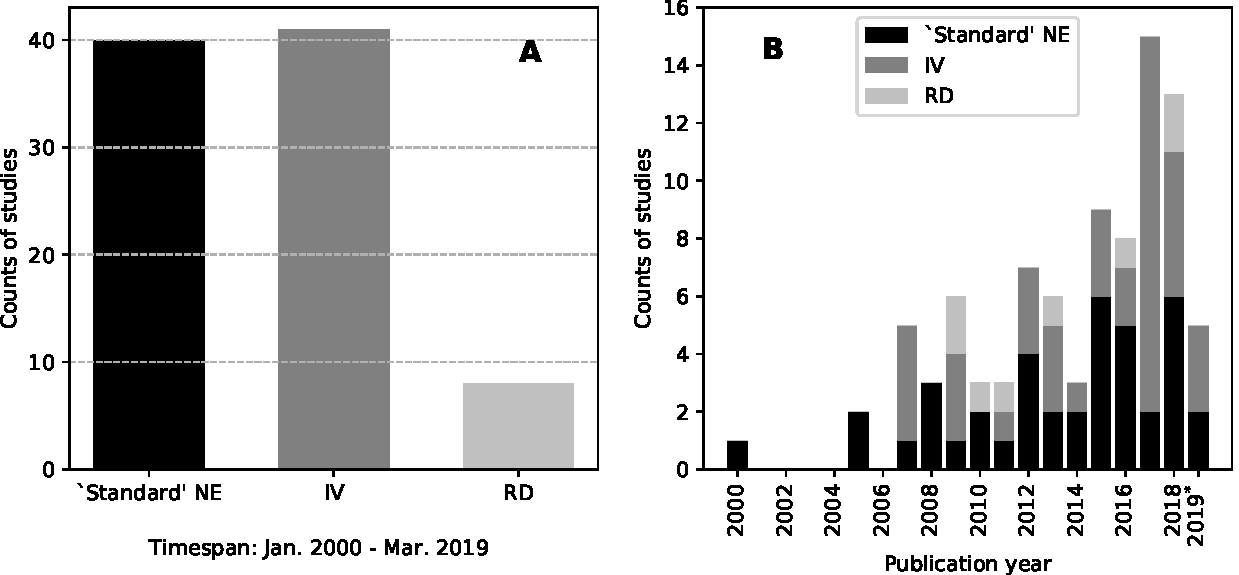
\includegraphics[width=1\textwidth]{_0}
	\label{fig:ne_studies_distr}
	\caption*{\textit{Notes.---}`Standard NE'
	denotes the group of studies that use an average treatment on the
	treated approach; `IV' denotes the group of studies using the
	instrumental variable design; `RD' denotes the group of studies using a
	regression discontinuity design. Panel `A' illustrates the group of
	studies across forms of NE experiments for the whole timespan; Panel `B'
	accounts for the formation of the stock data reported in Panel `A'.
	$^{*}$ `2019' data concern the first quarter of the year only. The
	number of individual studies is 87; Dal Bó et al. (2009) is included in
	both the IV and RD categories; Dasgupta (2018) is included both in the
	SNE and IV categories.}

\end{figure}

\subsection{Characterizing the Natural Experiment Studies}

\noindent As stated in the introduction, one of this paper's goals is to
understand `how' natural experiment methods intersect with substantive
topics in the field of leadership. In order to do this, we used topic
modeling---a text mining tool rooted in computational linguistics and
natural language processing\footnote{For a non-technical introduction to
  the topic see Mohr and Bogdanov (2013).}---to assess how the studies
retained map onto the topics dealt with in \emph{The Leadership
Quarterly}. In our case, a topic modeling approach has some advantages
over manually coding papers. First, it lets the `data speak' as the
study-to-topic pairing is revealed inductively by analyzing the corpus
of texts. Hence, the researcher does not need to subjectively assign a
study to an established, theoretically derived topic. Second, topic
modeling offers a nuanced characterization of the substantive focus of a
study. Not only is the assignment of a document to a topic
probabilistic, a document is also related to multiple topics. In other
words, an article that investigates the firm level implications of
gender diversity in top management teams may reflect both the `strategic
leadership' and `gender diversity in groups' categories that Gardner and
colleagues map.

\begin{sidewaystable}[!htbp]
	\centering
	\caption{Term-Topic Matrix}
	\label{tab:term_topics}
        \resizebox{0.85\textwidth}{!}{%
        \begin{threeparttable}
	\begin{tabular}{cccccccccccc}
	\toprule \toprule
	Topic Number & \multicolumn{10}{c}{Terms as Lemmas} \\  \\[-1.8ex] \cline{2-11}
	\\[-1.8ex]
	1   & context          & woman         & difference & power     & role
            & gender           & practice      & female     & culture   & position
           \\
            & ( 0.042 )        & ( 0.03 )      & ( 0.024 )  & ( 0.024 ) & ( 0.02 )   & ( 0.017 )  & ( 0.017 )   & ( 0.016 )   & ( 0.013 )   & ( 0.012 )      \\  \\ [-1.8ex] \\ [-1.8ex]
	2   & perception       & affect        & role       & emotion   & positive   & emotional  & negative    & network     & influence   & collective     \\
            & ( 0.034 )        & ( 0.033 )     & ( 0.03 )   & ( 0.028 ) & ( 0.028 )  & ( 0.026 )  & ( 0.026 )   & ( 0.017 )   & ( 0.016 )   & ( 0.016 )      \\  \\ [-1.8ex] \\ [-1.8ex]
	3   & transformational & subordinate   & rating     & trait     & associate  & experience & significant & personality & high        & analysis       \\
            & ( 0.056 )        & ( 0.043 )     & ( 0.026 )  & ( 0.021 ) & ( 0.017 )  & ( 0.016 )  & ( 0.016 )   & ( 0.016 )   & ( 0.014 )   & ( 0.014 )      \\  \\ [-1.8ex] \\ [-1.8ex]
	4   & development      & perspective   & develop    & political & include    & purpose    & interest    & view        & multiple    & year           \\
            & ( 0.046 )        & ( 0.027 )     & ( 0.017 )  & ( 0.015 ) & ( 0.015 )  & ( 0.013 )  & ( 0.013 )   & ( 0.012 )   & ( 0.012 )   & ( 0.01 )       \\  \\ [-1.8ex] \\ [-1.8ex]
	5   & employee         & work          & lmx        & job       & supervisor & perceive   & authentic   & mediate     & hypothesis  & satisfaction   \\
            & ( 0.054 )        & ( 0.048 )     & ( 0.034 )  & ( 0.023 ) & ( 0.023 )  & ( 0.021 )  & ( 0.019 )   & ( 0.018 )   & ( 0.016 )   & ( 0.015 )      \\  \\ [-1.8ex] \\ [-1.8ex]
	6   & understand       & effective     & vision     & problem   & cognitive  & strategy   & lead        & dynamic     & proposition & identify       \\
            & ( 0.024 )        & ( 0.02 )      & ( 0.019 )  & ( 0.017 ) & ( 0.017 )  & ( 0.015 )  & ( 0.014 )   & ( 0.013 )   & ( 0.013 )   & ( 0.013 )      \\  \\ [-1.8ex] \\ [-1.8ex]
	7   & performance      & team          & member     & ceo       & management & skill      & firm        & decision    & share       & strategic      \\
            & ( 0.106 )        & ( 0.085 )     & ( 0.033 )  & ( 0.03 )  & ( 0.021 )  & ( 0.019 )  & ( 0.018 )   & ( 0.018 )   & ( 0.017 )   & ( 0.015 )      \\  \\ [-1.8ex] \\ [-1.8ex]
	8   & level            & increase      & ethical    & develop   & impact     & moral      & structure   & reveal      & practice    & integrity      \\
            & ( 0.029 )        & ( 0.024 )     & ( 0.023 )  & ( 0.019 ) & ( 0.017 )  & ( 0.016 )  & ( 0.015 )   & ( 0.014 )   & ( 0.013 )   & ( 0.012 )      \\  \\ [-1.8ex] \\ [-1.8ex]
	9   & charismatic      & change        & manager    & time      & charisma   & style      & content     & crisis      & type        & managerial     \\
            & ( 0.051 )        & ( 0.041 )     & ( 0.035 )  & ( 0.03 )  & ( 0.025 )  & ( 0.018 )  & ( 0.014 )   & ( 0.013 )   & ( 0.012 )   & ( 0.01 )       \\  \\ [-1.8ex] \\ [-1.8ex]
	10  & group            & effectiveness & task       & condition & identity   & individual & emergence   & show        & response    & characteristic \\
            & ( 0.073 )        & ( 0.04 )      & ( 0.03 )   & ( 0.023 ) & ( 0.022 )  & ( 0.021 )  & ( 0.019 )   & ( 0.017 )   & ( 0.015 )   & ( 0.014 )      \\  \\ [-1.8ex] \\ [-1.8ex]
	\bottomrule
	\end{tabular}
	\begin{tablenotes}[flushleft]
	\item {\textit{Notes.---} Estimations achieved with Mallet
			software and the Gensim library for Python; number of
			documents = 1,156; number of topics = 10; terms are
			arranged in descending order of likelihood to appear in
			topic $i$; the optimal number of topics to retain is based
		        on the comparison and contrast of the coherence value of 29
                 	competing models in the 1-29 topics range---see Appendix
                        \ref{appendix_b} for further details about the estimation procedure.}
	\end{tablenotes}
	\end{threeparttable}}
\end{sidewaystable}

In terms of design, our topic modeling involves two phases. In the first phase
we trained a Latent Dirichlet Allocation ( LDA) model (Blei, Ng \& Jordan, 2003)
on the abstracts of the 1,156 research articles\footnote{Editorial notes were
not used to train the model.} published in the \emph{The Leadership Quarterly}
between January 2000 and March 2019. Table 1 illustrates key estimates obtained
using Mallet (McCallum, 2002) and the Gensim (Řehůřek \& Sojka, 2010) and spaCy
(Honnibal \& Montani, 2017) libraries for Python. Each cell in the table
indicates the probability of a term \(w\) (e.g., `CEO') of occurring in a topic
\(\tau\) (e.g., Topic 2). The analysis of the term-topic pairs included in the
model reveals a series of substantive categories that seem consistent with
Gardner and colleagues' review. The models emphasize topics such as `female
leadership' (Topic 1); `emotions and leadership' (Topic 2); `transformational
leadership' (Topic 3) `development of leadership' (Topic 4); `dyadic relations'
(Topic 5); `cognition and leadership' (Topic 6); `strategic leadership' (Topic
7); `ethical leadership' (Topic 8); `charismatic leadership' (Topic 9);
`leadership in team and decision groups' (Topic 10).

In the second phase, we used a folding-in strategy by `projecting' each of the
87 natural experiments onto the trained LDA model. We thus represented each
retained study in terms of the very same ten topics that represent the corpus of
1,156 abstracts published in \emph{The Leadership Quarterly} between January
2000 and March 2019. This enabled us to characterize a natural experiment in
terms of one or a few salient topics (i.e., those that occur with a higher
likelihood in the document) or to allocate it as being leadership research.
Appendix~\ref{appendix_b} provides further descriptive elements about the
estimation procedure behind our LDA model. The supplemental materials contain
the data and the Python code to reproduce the set of exhibits reported in the
paper.

\section{Literature Review}\label{sec:descriptive_part}

\subsection{Standard Natural Experiments}

\noindent The standard natural experimental design was used in the first-ever
natural experiment, in which Snow (1855) analyzed the transmission of
cholera in mid-19th century London. In its `simplest' form, the standard
natural experiment resembles the design of a randomized experiment in
that there are two groups---the treatment and control group with a pre-
and a post-treatment observation per group.\footnote{The standard
  natural experiment is also often referred to as the ``difference in
  difference (DID)'' design; however, not all DID designs represent
  natural experiments, e.g., if the assignment is based on
  self-selection or unobserved covariates and not on an as-if
  randomization (Wing et al., 2018).}

The standard natural experimental design was already used in the first-ever
natural experiment, in which Snow (1855) analyzed the transmission of cholera in
London. In its `simplest' form, the standard natural experiment resembles the
design of a randomized experiment in that there are two groups---the treatment
and control group---with two observations per group---a pre- and a
post-treatment observation.\footnote{The standard natural experiment is also
	often referred to as ``difference in difference (DID)'' design; yet, not
all DID designs represent natural experiments, e.g., if the assignment is based
on self-selection or unobserved covariates and not on an as-if randomization
(Wing et al., 2018).} As shown in Figure~\ref{fig:sne}, we can estimate the
causal effect of the treatment by comparing the average change of the outcome
variable $y$ for the treated units ($\lambda + \delta$) and controls ($\gamma$).
Of course, the `simple' form of the standard natural experiment can be extended
in several ways, such as by adding additional treatment groups or by adding
additional time periods before and/or after the treatment (e.g., Matsa and
Miller, 2013).

\begin{figure}[] 
	\centering
	\caption{Visual Representation of the Standard Natural Experiment}
	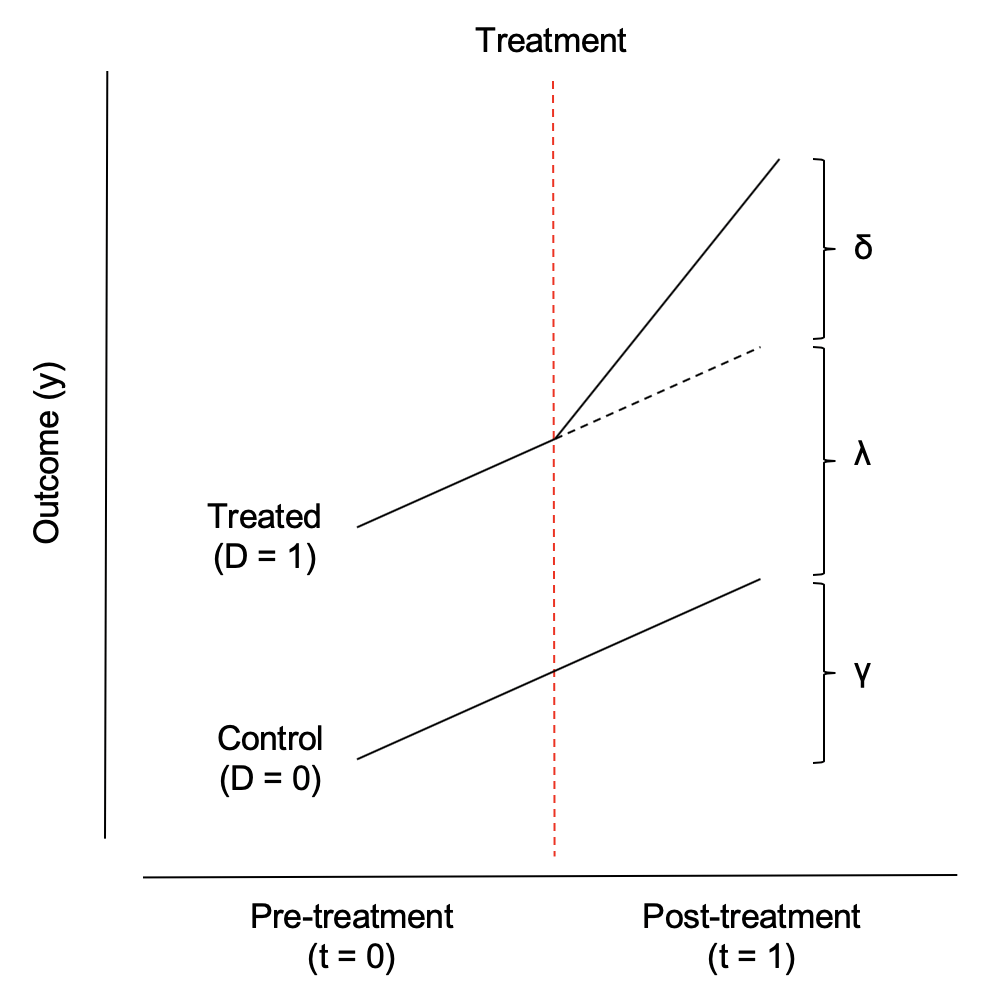
\includegraphics[width=0.5\textwidth]{_4}
	\label{fig:sne}
	\caption*{\textit{Notes.---}The underlying population regression
		function is $y = \gamma t + \lambda D + \delta t D$, where
		$\gamma$, $\lambda$, and $\delta$ represent the systematic
		difference in the outcome across the treated and control cases,
		the trend effect and the difference in the outcome that is due
	to the treatment. For sake of clarity we represent the case in which
$\delta > 0$.}
\end{figure}

Whether the standard natural experiment provides a causal estimate
mainly depends on the qualities of the treatment. In the case of random
variations, such as lotteries, the assignment process needs to be truly
random (e.g., Starr, 1997). In the case of as-if random variations, the
assignment process needs to be independent of factors that are related
to the outcome and not affected by the unit's self-selection into
treatment or control conditions (Dunning, 2012). The second part of the
document deals with these aspects in more detail.


\subsubsection{Standard Natural Experiment and Leadership Research}

\noindent Table~\ref{tab:sne_list} reports the set of studies that draw upon the
standard natural experiment design to address a leadership-related topic. The
left-hand column indicates the short reference for the study; the remaining
columns provide a substantive characterization of the study. The right-hand
columns present the inductive categorization of studies as emerging from the
topic modeling described in the previous section. In the interest of clarity, we
have just reported the two most salient topics of each study---i.e., the topics
with the highest chance of being paired with the focal document.

Our topic model highlights the focus of the standard natural experiments and
consists of three core topics---`female leadership' (Topic 1); `strategic
leadership' (Topic 7); and `ethical leadership' (Topic 8)---together with a
series of other themes that, although less central, still receive significant
attention (see Topics 2, 3, 4, 6, 9, and 10).  The prominence of Topics 1, 7 and
8 is clear from Figure~\ref{fig:mds_ne}, Panel A, which shows the frequency with
which salient topics appear in the documents.

The scatter plot in Panel B of Figure~\ref{fig:mds_ne} expands on the outcome
of the topic model by positioning each natural experiment in the topic space
that characterizes the population of articles published in \emph{The Leadership
Quarterly}. The coordinates of each data point are produced via multidimensional
scaling. This allows us to create a shallow representation of the 10-dimension
space underlying the topic model.  `Stars' are associated with natural
experiments. \emph{The} \emph{Leadership Quarterly} articles are represented
with circles that have been color-coded to reflect the dominant topic of the
document. The diagram highlights that: (i) standard natural experiments map onto
a narrow portion of the space, whereas vast areas of leadership research have
been barely or not impacted at all by this form of causal research; (ii) an
initial cluster of studies emerges at the intersection of `female leadership'
and strategic leadership (see the bottom right of the chart); (iii) a second
cluster of studies jointly investigate `ethical leadership' and `nature of
managerial work' subjects (see the middle left of the chart).	 

\begin{table}[!htbp]
	\centering
	\caption{Standard Natural Experiments---Substantive Focus}
	\label{tab:sne_list}
	\resizebox{1\textwidth}{!}{%
	\begin{tabular}{{@{\extracolsep{5pt}}l  l D{.}{.}{5} l D{.}{.}{5}}}
		\toprule \toprule
		\multicolumn{1}{c}{}                &
		\multicolumn{4}{c}{Salient topics} \\ \\[-1.8ex]
		\cline{2-5} \\[-1.8ex]
		&
		\multicolumn{2}{c}{$1^{st}$ topic}  &
		\multicolumn{2}{c}{$2^{nd}$ topic}  \\ \\[-1.8ex]
		\cline{2-3} \cline{4-5} \\[-1.8ex]
		\multicolumn{1}{c}{Study} &
		\multicolumn{1}{c}{Topic label}        &
		\multicolumn{1}{c}{Prob.}           &
		\multicolumn{1}{c}{Topic label}        &
		\multicolumn{1}{c}{Prob.}           \\
		\midrule
              Bae \& Yi (2008) &                   Charismatic leadership &     0.134 &                       Ethical leadership &     0.133 \\
         Beaman et al. (2012) &              Transformational leadership &       0.2 &                        Female leadership &     0.165 \\
         Belloc et al. (2016) &                 Cognition and leadership &     0.143 &                Development of leadership &     0.134 \\
              Bhavnani (2017) &                   Charismatic leadership &     0.165 &                        Female leadership &     0.148 \\
            Breda \& Ly (2015) &                        Female leadership &     0.204 &                  Emotions and leadership &     0.148 \\
       Brockman et al. (2015) &                     Strategic leadership &     0.332 &                       Ethical leadership &     0.102 \\
           Byrd et al. (2012) &                     Strategic leadership &     0.174 &                        Female leadership &     0.165 \\
              Bækgaard (2011) &  Leadership in teams                    &      0.18 &                        Female leadership &     0.167 \\
             Chauchard (2014) &                        Female leadership &     0.137 &  Leadership in teams &     0.127 \\
           Chen et al. (2016) &                     Strategic leadership &     0.181 &                        Female leadership &     0.171 \\
          Cheng et al. (2005) &                     Strategic leadership &     0.173 &                Development of leadership &     0.113 \\
          Cohen \& Wang (2013) &  Leadership in teams &     0.139 &                Development of leadership &     0.128 \\
                 Coman (2018) &                Development of leadership &     0.149 &                        Female leadership &     0.131 \\
            Cox et al. (2000) &                     Strategic leadership &     0.155 &  Leadership in teams  &      0.14 \\
     Cuñat \& Guadalupe (2009) &                     Strategic leadership &     0.194 &                       Ethical leadership &     0.159 \\
     Dahya \& McConnell (2005) &                        Female leadership &     0.227 &                  Emotions and leadership &     0.108 \\
              Dasgupta (2018) &                        Female leadership &     0.123 &                   Charismatic leadership &     0.119 \\
           De \& Scoppa (2015) &                        Female leadership &     0.233 &  Leadership in teams &     0.125 \\
             De et al. (2010) &                        Female leadership &     0.322 &                 Cognition and leadership &     0.104 \\
        Gittell et al. (2008) &                         Dyadic relations &      0.18 &                  Emotions and leadership &      0.13 \\
        Gormley et al. (2012) &                     Strategic leadership &     0.202 &                   Charismatic leadership &     0.135 \\
      Guadalupe \& Wulf (2010) &                     Strategic leadership &     0.179 &                       Ethical leadership &     0.127 \\
           Han \& Zhang (2018) &                        Female leadership &     0.194 &                     Strategic leadership &     0.155 \\
        Hidalgo et al. (2016) &                        Female leadership &     0.186 &                  Emotions and leadership &     0.126 \\
     Huber \& Arceneaux (2007) &                   Charismatic leadership &     0.214 &                       Ethical leadership &     0.136 \\
  Jayaraman \& Milbourn (2015) &                     Strategic leadership &     0.274 &                  Emotions and leadership &     0.109 \\
        Jiraporn \& Lee (2018) &                        Female leadership &     0.205 &                Development of leadership &     0.113 \\
       Jiraporn et al. (2018) &                        Female leadership &      0.19 &                       Ethical leadership &     0.128 \\
           Kahn et al. (2015) &                 Cognition and leadership &     0.157 &                        Female leadership &     0.141 \\
   Laustsen \& Petersen (2017) &                Development of leadership &      0.15 &                 Cognition and leadership &     0.128 \\
          Matsa et al. (2013) &                        Female leadership &     0.224 &                     Strategic leadership &     0.177 \\
                Poulos (2019) &                        Female leadership &     0.169 &                       Ethical leadership &     0.126 \\
        Rickman \& Witt (2008) &              Transformational leadership &     0.128 &                     Strategic leadership &     0.122 \\
          Shea \& Solis (2018) &                       Ethical leadership &     0.127 &                        Female leadership &      0.12 \\
                Siming (2016) &                        Female leadership &     0.161 &                 Cognition and leadership &     0.158 \\
        Tabvuma et al. (2014) &                   Charismatic leadership &     0.138 &                        Female leadership &     0.128 \\
                 Tosun (2016) &                     Strategic leadership &     0.238 &                       Ethical leadership &     0.118 \\
               Valdini (2012) &                        Female leadership &     0.271 &              Transformational leadership &     0.115 \\
            Vo \& Canil (2019) &                     Strategic leadership &     0.217 &                       Ethical leadership &     0.134 \\
               Wyrwich (2015) &              Transformational leadership &     0.165 &                 Cognition and leadership &     0.154 \\
		\bottomrule
       \end{tabular}}
%		\caption*{\small{\textit{Notes.---}Topic labels: Topic
%				1---`female leadership'; Topic
%				2---`emotions and leadership \& gender'; Topic
%				3---transformational leadership'; Topic
%				4---`development of leadership'; Topic 5---`(neo-)charismatic
%				leadership'; Topic 6---`complexity approaches
%				to leadership'; Topic 7---`ethical and moral
%				leadership'; Topic 8---`leadership
%				development'; Topic 9---`nature of managerial
%				work'; Topic 10---`leadership in teams and
%		decision group.'}}
\end{table}


\begin{figure}
	\centering
	\caption{Standard Natural Experiments---Topic Characterization}
	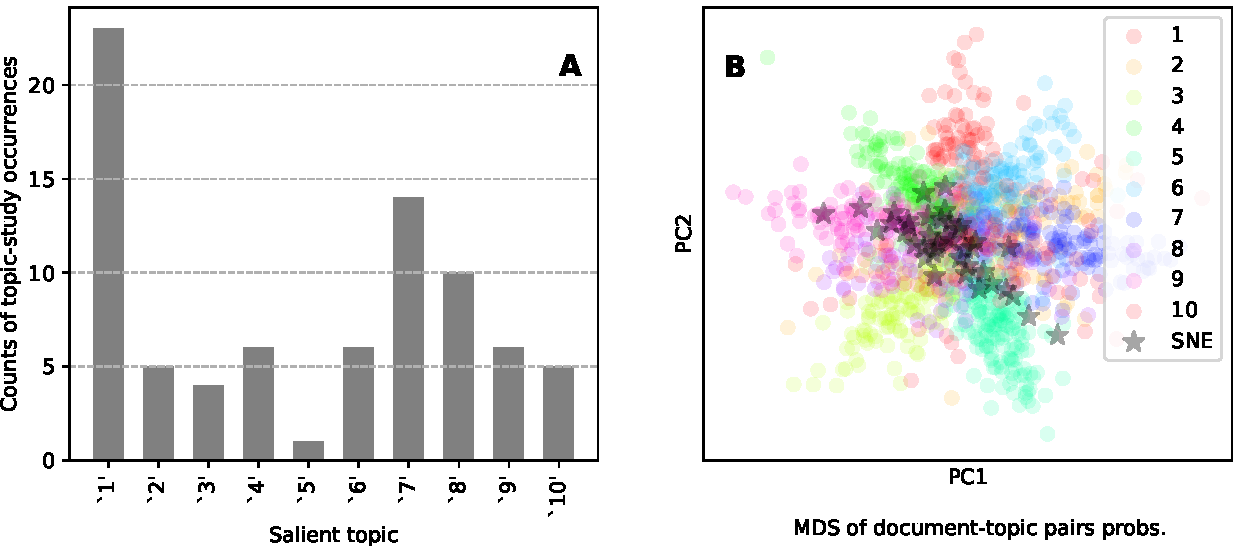
\includegraphics[width=1\textwidth]{_1}
	\label{fig:mds_ne}
	\caption*{\small\textit{Notes.---} Panel A pictorially depicts the
		information reported in Table~\ref{tab:sne_list}; Panel B: Data points
		marked with a star denote natural experiments that are folded
		in the topic model trained on the 1,156 articles published in The
		Leadership Quarterly; Topic labels: Topic 1---`female
		leadership'; Topic 2---`emotions and leadership';
		Topic 3---transformational leadership'; Topic 4---`development
		of leadership'; Topic 5---`(neo-)charismatic leadership'; Topic
		6---`cognition and leadership'; Topic 7---`strategic
		leadership'; Topic 8---`ethical leadership'; Topic 9---`nature
		of managerial work'; Topic 10---`leadership
		in teams and decision group.' `MDS' stands for
		multdimensional scaling; `PC1' and `PC2' refer to the
components returned from the MDS analysis.}
\end{figure}


\subsubsection{Standard Natural Experiment Examples}

\noindent Our review shows there is a significant number of studies using standard
natural experiments to address selected leadership-related topics. We
concentrate on three examples in order to provide leadership scholars
with insights into the application of the standard natural experiment
for inferring causal relationships.

The first study, by Beaman and colleagues (2012), uses a standard
natural experiment to analyze whether female leadership has an impact on
girls' career aspirations and educational attainment. The authors
hypothesize that a female leader will act as a role model for girls and
young women, and will thereby affect their career aspirations and
educational attainment. The authors argue that analyzing this
relationship in laboratory experiments is difficult, because
participants are exposed to the role model for a short period of time,
whereas in observational studies, people may self-select to certain role
models based on observed and unobserved characteristics. Beaman and
colleagues (2012) thus exploit the enactment of a law in India in 1993
that determined that in some randomly selected villages, the position of
chief councilor was reserved for women. The law resulted into two
treatment groups and a control group. The first treatment group consists
of villages in which this position was reserved for women in one
election (either 1998 or 2003); in the second treatment group, the
position was reserved for women in two elections (in 1998 and 2003); and
in the control group, the position was never reserved for women. The
authors collected survey data from 15 randomly selected households in
each village in 2006 and 2007. Their difference-in-means analyses show
that the gender gap in parents' career aspirations for their children
was much lower in villages in which the council positions had been
reserved for women twice compared to villages in which the position had
been reserved for women once or never. The analyses also indicate that
the gap in educational aspirations between boys and girls was much lower
in villages with female leaders than in villages with male leaders.
Based on some additional analyses, the authors conclude that the effects
are mainly caused by a role model effect; that is, female leaders
provide a role model both for parents and for girls. Overall, the
standard natural experiment by Beaman and colleagues (2012) provides
important insights into the causal effect of female leadership on
(female) followers' aspirations.

In the second study, Matsa and Miller (2013) exploit the introduction of
`gender quota' policies in Norway to investigate how female leadership
influences strategic choices and outcomes, for example corporate
downscaling. The gender quotas forced all publicly listed firms in
Norway to increase the proportion of women on the board of directors to
40\% within two years. Because the gender-quota policy applied to all
listed firms, it was not a random variation in the regulatory
environment. However, the authors argue that the policy targets
companies that are part of a broader population of Scandinavian firms,
that is, organizations facing relatively similar cultural and
institutional factors. The Norwegian policy may therefore have an
as-if-random interpretation. Matsa and Miller (2013) used a matching
approach in which they first pair treated (i.e., publicly listed) and
untreated (i.e., unlisted) Norwegian firms, and, in the second step,
linked Norwegian firms to listed and unlisted firms located in Denmark,
Finland, and Sweden. The summary statistics showed that the treatment
and control group were similar in terms of most firm characteristics. To
analyze the causal effect of female leadership on strategic choices and
outcomes, the authors used the difference-in-differences and
difference-in-difference-in-differences\footnote{The
  difference-in-difference-in-differences framework is also referred to
  as the `triple diff-in-diffs.'} analytical frameworks. They found that
the gender quota had a negative impact on firm profitability. In further
analyses, the authors showed that profit differentials were mainly
attributable to the fact that companies treated with the quota policy
tended to cut less jobs than their counterparts. To back up the causal
interpretation of their results, Matsa and Miller (2013) conducted
several robustness checks, such as testing for trends before the
introduction of the quota and testing whether the effects were stronger
for firms with fewer women on their board of directors. Overall, the
study provides causal empirical evidence supporting the effect of female
leadership on firm performance as mediated by key strategic choices.

The third study, by Shea and Solis (2018), analyzes the relationship
between leader tenure and countries' creditworthiness. The authors argue
that higher leader tenure will reduce uncertainty in the sovereign
credit market and will therefore increase a country's creditworthiness.
Since leader tenure is endogenous (e.g., effective leaders tend to have
a higher tenure), the authors backup their panel data analysis with a
natural experiment in which leader tenure is exogenously determined.
They focused on countries characterized by attempts to assassinate the
political leader. While such events are not random, as confirmed by the
authors' balance tests (see also the discussion in Jones and Olken,
2005), the outcome is as-if random. The authors provide anecdotal
evidence for this claim (e.g., the successful assassination of President
Kennedy versus the unsuccessful assassination of President Reagan) and
excluded all assassinations in which the success was not determined by
chance (e.g., \emph{en coup d'etat}). Shea and Solis (2018) used a
two-step approach in their analysis. First, they regressed sovereign
bond yields on leader tenure, assassination success, and an interaction
term. The interaction term was positive and significant, which indicated
that assassination success had a stronger effect on bond yields at
higher levels of leader tenure. Second, the authors accounted for a
potential selection in the assassination sample (i.e., assassination
attempts are likelier in poorer, non-democratic states) by applying the
Heckman selection model, which supported the findings from the OLS.
Overall, the study used an unusual exogenous variation of leader tenure
to provide robust evidence that leader tenure influences a country's
creditworthiness.

To sum up, the three examples of standard natural experiments explore
important leadership topics (e.g., consequences of a leader's tenure and
female leadership) and provide robust causal inference. The three
studies use very different exogenous variations, such as laws or even
assassination attempts, and focus on leadership in the contexts of
villages, firms, and states. Thus, the three examples highlight both the
potential and the variability of standard natural experiments for
leadership research.


\subsection{Instrumental Variable Designs} 

\noindent Instrumental variable (IV) designs have already received some attention
in management research, as several researchers recommend their use to
correct for endogeneity in the relationship between an independent
variable and a dependent variable (e.g., Bascle, 2008; Semadeni et al.,
2014). The basic idea of the IV design is shown in Figure~\ref{fig:iv_path}: The
treatment variable $D$ is influenced by covariates $A$, $B$, and
$F$. Because at least one of the covariates is unobserved, we cannot
directly estimate the causal effect of the treatment $D$ on the
outcome $Y$. The IV design `solves' the endogeneity problem, which
results from the omitted variable bias, by leveraging an instrument
$C$ to which subjects are (as-if) randomly assigned (Dunning, 2012).

A valid instrument needs to fulfill three conditions (Angrist \&
Pischke, 2009). First, it needs to be exogenous, which means that it is
uncorrelated with other causes of the dependent variable except for the
treatment. Second, the instrument needs to influence the assignment of
the treatment (i.e., it influences the probability of receiving the
treatment). Third, the instrument has no relationship with the dependent
variable except through the treatment. A violation of the conditions can
lead to a severe bias in the estimates (Bound, Jaeger, \& Baker, 1995;
Semadeni et al., 2014). It is therefore important that researchers
thoroughly scrutinize any candidate instrument and check whether and to
what extent it fulfills these three conditions.

\begin{figure}[!htbp]
	\centering
	\caption{Visual Representation of the Instrumental Variable Framework}
	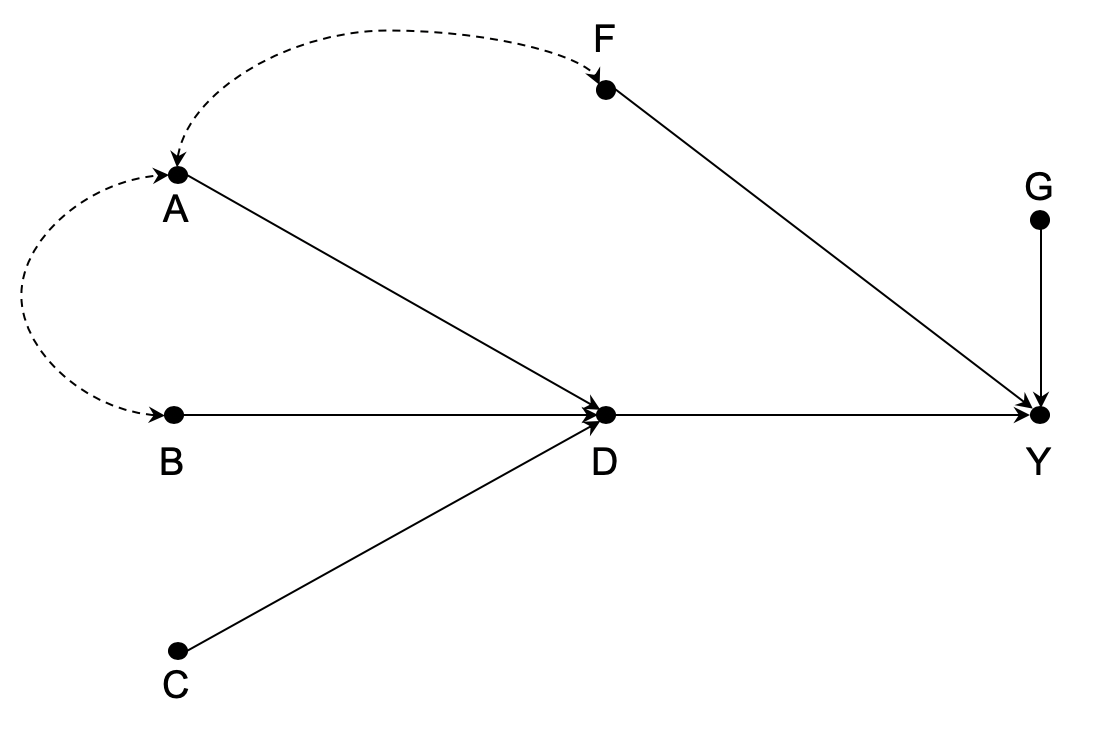
\includegraphics[width=0.55\textwidth]{_5}
	\label{fig:iv_path}
	\caption*{\textit{Notes.---} Continuous, oriented arrows denote the
		causal effect linking two variables; Dashed edges denote the
		presence of a common cause between two variables; $C$ is an
		instrumental variable for $D$; $A$, $B$, and $F$ are
		observables that influence $D$; $G$ is a variable that affects
		the outcome but it is not causally related to $D$, so it does
not affect the presumed causal path linking $D$ to $Y$; Source: Morgan and
Winship (2015, page 30).}
\end{figure} 

 
\subsubsection{Instrumental Variable Designs and Leadership Research}

\noindent Table~\ref{tab:iv_list} reports the set of studies that draw upon the
IV design. Our topic model---whose insights are summarized in Figure 5, Panel
A---reveals that `female leadership' (Topic 1) and `strategic leadership' (Topic
7) tend to dominate the focus of attention of this group of studies. In fact,
the core topics are even more core in this case than in standard natural
experiments, whereas the number of documents that build on the remaining topics
is relatively small. Panel B, showing the positioning of IV designs in terms of
the articles published in \emph{The Leadership Quarterly}, confirms that the
data-points are concentrated in the bottom right of the chart.


\begin{table}[!htbp] 
	\centering
	\caption{Instrumental Variables Designs---Substantive Focus}
	\label{tab:iv_list}
	\resizebox{1\textwidth}{!}{%
	\begin{tabular}{{@{\extracolsep{5pt}}l l D{.}{.}{5} l D{.}{.}{5}}}
		\toprule \toprule
		\multicolumn{1}{c}{}                &
		\multicolumn{4}{c}{Salient topics} \\ \\[-1.8ex]
		\cline{2-5} \\[-1.8ex]
		&
		\multicolumn{2}{c}{$1^{st}$ topic}  &
		\multicolumn{2}{c}{$2^{nd}$ topic}  \\ \\[-1.8ex]
		\cline{2-3} \cline{4-5} \\[-1.8ex]
		\multicolumn{1}{c}{Study} &
		\multicolumn{1}{c}{Topic label}        &
		\multicolumn{1}{c}{Prob.}           &
		\multicolumn{1}{c}{Topic label}        &
		\multicolumn{1}{c}{Prob.}           \\
		\midrule
         Adams et al. (2009) &         Strategic leadership &     0.214 &                        Female leadership &     0.113 \\
             Adhikari (2018) &            Female leadership &     0.177 &                     Strategic leadership &     0.134 \\
        Adkins et al. (2007) &         Strategic leadership &     0.162 &                        Female leadership &     0.134 \\
        Aghion et al. (2013) &         Strategic leadership &     0.151 &                        Female leadership &     0.148 \\
        Akyol \& Cohen (2013) &            Female leadership &     0.186 &                     Strategic leadership &     0.181 \\
         Amore et al. (2014) &            Female leadership &     0.181 &                     Strategic leadership &     0.142 \\
         Amore et al. (2017) &         Strategic leadership &     0.156 &              Transformational leadership &     0.122 \\
                Arora (2018) &            Female leadership &     0.176 &                     Strategic leadership &     0.144 \\
          Artz et al. (2017) &  Transformational leadership &     0.185 &                         Dyadic relations &     0.163 \\
       Azoulay et al. (2017) &  Transformational leadership &     0.139 &                Development of leadership &     0.135 \\
       Barros \& Nunes (2007) &         Strategic leadership &     0.136 &                       Ethical leadership &     0.134 \\
     Bennedsen et al. (2007) &         Strategic leadership &     0.283 &              Transformational leadership &     0.181 \\
       Bernile et al. (2018) &            Female leadership &     0.179 &                       Ethical leadership &     0.171 \\
          Chen et al. (2017) &            Female leadership &     0.226 &                Development of leadership &     0.127 \\
   Chintrakarn et al. (2017) &     Cognition and leadership &     0.156 &                     Strategic leadership &     0.144 \\
      Conroy \& Weiler (2016) &         Strategic leadership &     0.219 &                        Female leadership &      0.14 \\
          Conyon \& He (2017) &         Strategic leadership &     0.198 &                        Female leadership &     0.191 \\
           Dal et al. (2009) &            Female leadership &     0.208 &                Development of leadership &     0.179 \\
             Dasgupta (2018) &            Female leadership &     0.123 &                   Charismatic leadership &     0.119 \\
         Delis et al. (2017) &            Female leadership &     0.239 &                     Strategic leadership &     0.139 \\
      Driver \& Guedes (2017) &         Strategic leadership &     0.155 &                Development of leadership &     0.144 \\
       Frantz \& Stein (2017) &            Female leadership &     0.151 &                     Strategic leadership &     0.138 \\
       Gabel \& Scheve (2007) &            Female leadership &     0.141 &                Development of leadership &     0.121 \\
      Harjoto \& Rossi (2019) &            Female leadership &      0.15 &                     Strategic leadership &     0.124 \\
  Hearn \& Filatotchev (2019) &           Ethical leadership &     0.156 &                        Female leadership &     0.128 \\
  Hooghiemstra et al. (2017) &            Female leadership &     0.141 &                     Strategic leadership &     0.132 \\
         Izgi \& Akkaş (2012) &         Strategic leadership &     0.203 &                        Female leadership &     0.151 \\
               Khwaja (2009) &         Strategic leadership &      0.17 &                        Female leadership &     0.126 \\
        Kılıç \& Kuzey (2016) &            Female leadership &     0.232 &                     Strategic leadership &     0.174 \\
            Li et al. (2018) &         Strategic leadership &      0.19 &              Transformational leadership &     0.156 \\
           Lin et al. (2011) &         Strategic leadership &     0.189 &                 Cognition and leadership &     0.183 \\
     Markussen \& Røed (2017) &            Female leadership &     0.196 &              Transformational leadership &     0.148 \\
      Nicolosi \& Yore (2015) &         Strategic leadership &     0.203 &                        Female leadership &     0.129 \\
        Pascal et al. (2017) &         Strategic leadership &     0.209 &                        Female leadership &     0.172 \\
                Rouse (2012) &  Transformational leadership &     0.167 &                     Strategic leadership &     0.128 \\
             Sabatier (2015) &            Female leadership &     0.165 &                       Ethical leadership &     0.138 \\
          Shue et al. (2017) &         Strategic leadership &     0.172 &                  Emotions and leadership &     0.167 \\
          Sun \& Hovey (2013) &         Strategic leadership &     0.273 &                        Female leadership &     0.115 \\
           Yang et al. (2019) &            Female leadership &     0.186 &                  Emotions and leadership &     0.144 \\
                   Wu (2015) &            Female leadership &     0.175 &                       Ethical leadership &     0.124 \\
                   de Vries (2012) &  Transformational leadership &     0.234 &  Leadership in teams &     0.219 \\
		\bottomrule
\end{tabular}}
\end{table}


\begin{figure}[!htbp] 
	\centering
	\label{fig:iv_mds}
	\caption{Instrumental Variable Designs---Topic Characterization}
	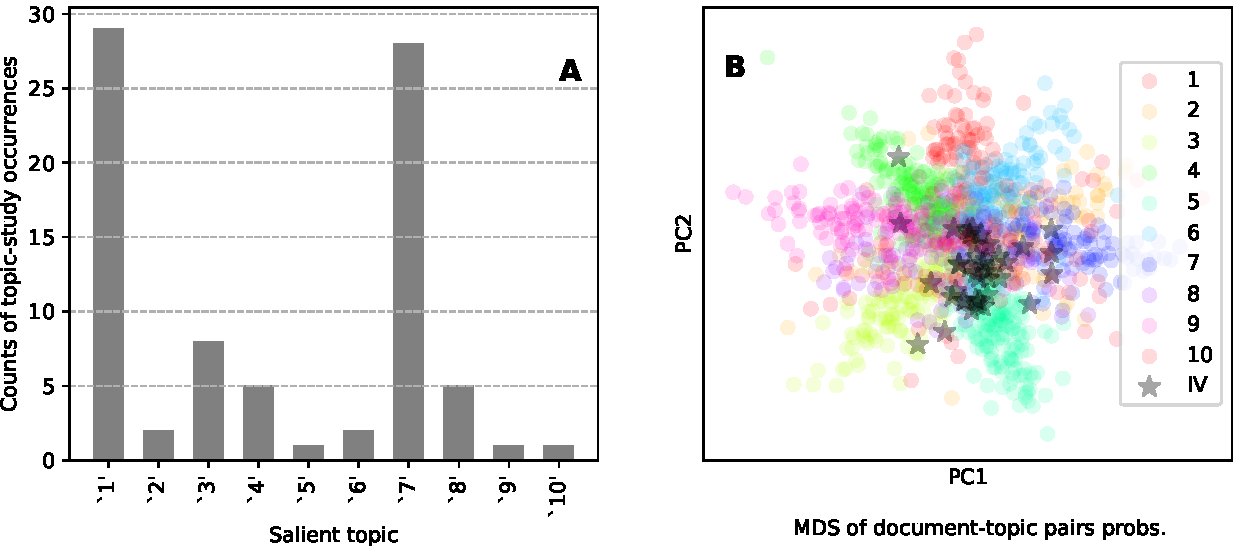
\includegraphics[width=1\textwidth]{_2}
	\caption*{\small\textit{Notes.---} Panel A pictorially depicts the
		information reported in Table~\ref{tab:iv_list}; Panel B: Data points
		marked with a star denote natural experiments that are folded
		in the topic model trained on the 1,156 articles published in The
		Leadership Quarterly; Topic labels: Topic 1---`female
		leadership'; Topic 2---`emotions and leadership';
		Topic 3---transformational leadership'; Topic 4---`development
		of leadership'; Topic 5---`(neo-)charismatic leadership'; Topic
		6---`cognition and leadership'; Topic 7---`strategic
		leadership'; Topic 8---`ethical leadership'; Topic 9---`nature
		of managerial work'; Topic 10---`leadership
		in teams and decision groups.' `MDS' stands for
		multdimensional scaling; `PC1' and `PC2' refer to the
components returned from the MDS analysis.}
\end{figure}


\subsubsection{Instrumental Variable Design Examples}

\noindent Our review shows that several studies in leadership research have
applied the IV design, but only to address very few topics. In this
section, we will focus on three example studies and explain their
approach in more detail in order to provide leadership scholars with
insights into how the IV design can be applied.

The first study was conducted by Bennedsen and colleagues (2007). It
analyzed the relationship between CEO succession decisions, particularly
the decision of family firms to hire a family or an external CEO, and
firm performance. Testing the causal effect of CEO succession decisions
on firm performance is difficult, because family members have in-depth
knowledge regarding the characteristics of other family members (e.g.,
human capital), which will probably affect their decision to hire an
external candidate. To infer a causal relationship, the authors use the
gender of the departing family CEO's firstborn child as an instrument.
They provide evidence that (i) the instrument is exogenous, because
gender is randomly assigned; (ii) the instrument is relevant, because in
the case of a family transition, it is about 10\% higher when the
firstborn child is male; and (iii) the instrument is unlikely to affect
firm performance through other channels than CEO succession decisions,
because a first child's gender is not related to firm-level attributes
(e.g., age, size, and profitability). The authors conducted supplemental
statistical analyses (e.g., using CEO deaths as an alternative
instrument; ruling out changes in governance structure as alternative
explanations) to back up their finding that appointing a family CEO
leads to a decline of ca. $4\%$ in firm profitability. Overall, the
study adopts a creative instrument to estimate the causal impact of
hiring professional managers on firm-level outcomes.

In the second study, Yang et al. (2019) investigated the relationships
between students' centrality within a social network, gender, and
attainment of leadership positions. The authors apply a two-study design
in which they first test their hypotheses based on observational data,
then infer the causal relationship by means of an IV design. The
correlational study shows that a student's ego-network is related to her
or his job placement in leadership positions. Network centrality is
positively related to job placement both for male and female
students---however, female students especially benefit from more
women-dominated networks and from relatively even communication with
peers. Because the observational study provides no insights into the
causal focal relationship, the authors exploit an exogenous variation in
the context. When students start their MBA program, they are randomly
assigned to home sections. Students take their first-quarter classes
only with students from their home section, which is why their
home-section-mates initially represent their most important friends.
Later in their studies, students bid for second-quarter classes. Since
the enrollment of students into classes is relatively unpredictable
(i.e., many students even end up in classes they did not bid for),
students have limited influence on the inter-personal ties they will
develop. The authors used a student's degree of exposure to same-gender
classmates from other home sections as the instrument. The findings of
the IV design mostly support the correlational study. Female students'
job placements are influenced by having an inner circle, whereas no
effect was found for male students. Overall, the study exploits the
as-if random assignment of students to networks as an instrument to
estimate the causal effect of networks on attaining leadership
positions, particularly for female leaders.

Finally, Chintrakarn et al. (2017) investigated the relationship between
managers' religious piety and firms' anti-takeover provisions. For the
instrument, the authors used the degree of religious piety from 1971 in
the community surrounding a company's headquarters. First, the authors
regressed the number of anti-takeover defenses on the non-instrumented
current religious piety variable and found a positive effect. In the
second step, they analyzed the same relationship based on instrumented
values of current religious piety. The two-stage least squares analysis
supported the conclusion of the correlational analysis that current
religious piety affects corporate governance, although the coefficient
of the instrumented treatment variable was smaller (b = 0.849) than the
coefficient of the non-instrumented treatment variable (b = 1.256). As a
robustness check, the authors used another instrumental variable---the
degree of religious piety in the population in 1952. The result of the
two-stage least squares supported the prior findings. Overall, the
authors provide evidence that religious piety substitutes for corporate
governance and reduces the conflict between managers and shareholders.

To sum up, the three examples highlight creative ways of applying
instruments to estimate causal relationships involving a variety of
leadership topics---including the consequences of leader selection for
firms (Bennedsen et al., 2007), leadership development (Yang et al.,
2019), and the consequences of culture on strategic leadership
(Chintrakan et al., 2017).


\subsection{Regression Discontinuity Design} 

\noindent The Regression Discontinuity (RD) design was initially developed by
Thistlethwaite and Campbell (1960). It capitalizes on the fact that in many
settings (e.g., business and education) a unit's score---above or below a
certain threshold on a continuous variable---determines the treatment status of
the unit. The basic idea of the RD design is shown in Figure~\ref{fig:rdd}.
When the assignment variable $X$ is greater than or equal to
$x^{*}$, which represents the threshold, units receive the treatment; if $X$ is
smaller than $x^{*}$, units receive no treatment. The RD design builds on the
assumption that in the neighborhood of the threshold ($x^{*}$) the  assignment
process is almost random (Dunning, 2012; Lee \& Lemieux, 2010). Then, the
variance in the outcome variable $y$ across the $X < x^{*}$ and $X \geq x^{*}$
regimes is caused by the treatment (Antonakis et al., 2010), represented by the
quantity $\delta$.

\begin{figure}[!htbp]
	\centering
	\caption{Visual Representation of the Regression Discontinuity Design}
	\label{fig:rdd}
	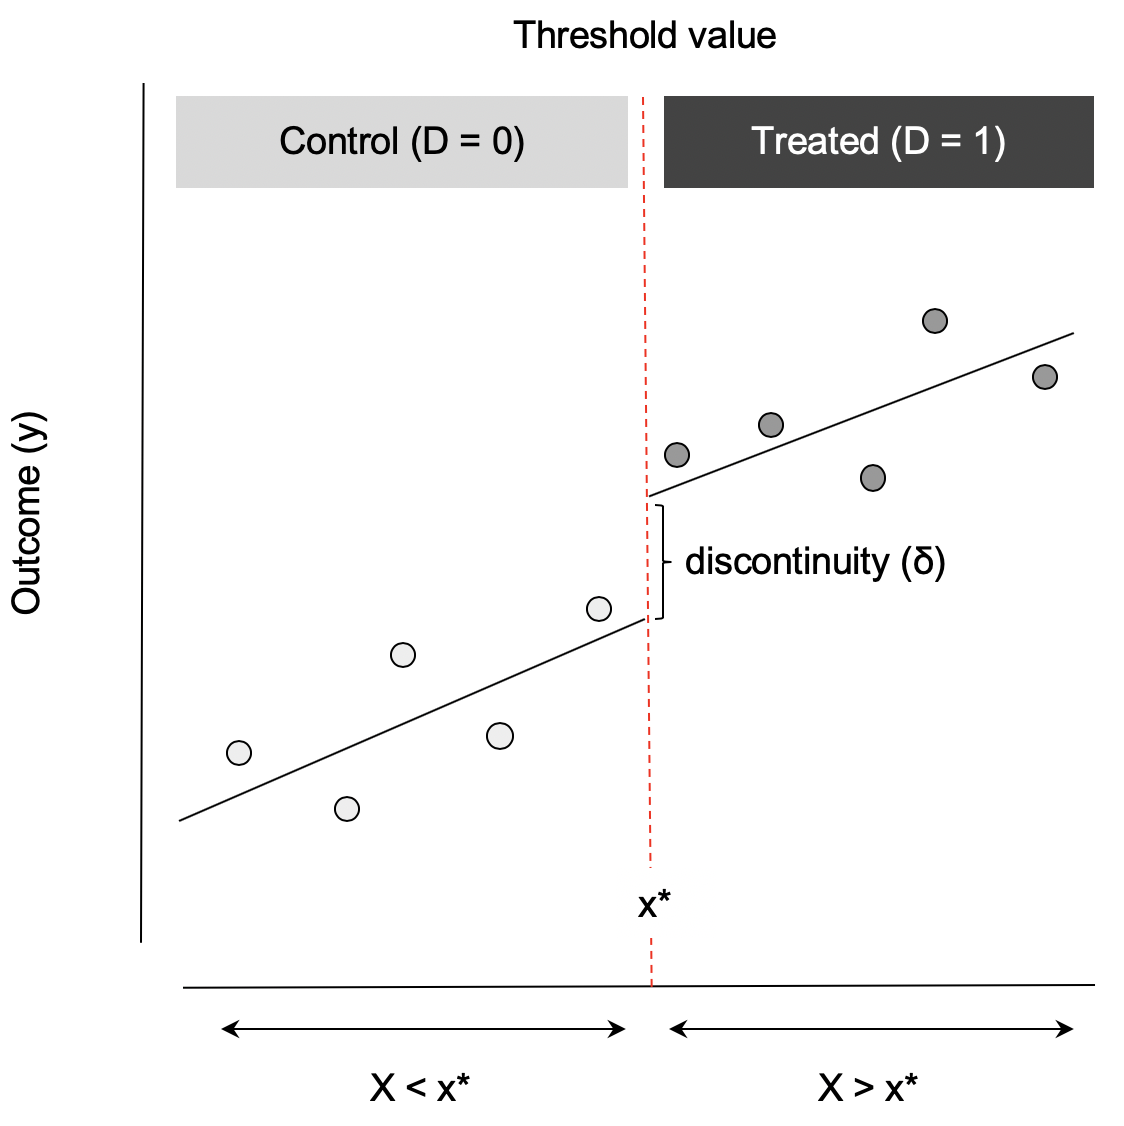
\includegraphics[width=0.55\textwidth]{_6}
	\caption*{\textit{Notes.---}The underlying population regression
	function is $y = \alpha + \delta  D + \beta(X-x^{*})$, where $y$ is
the response variable, $\alpha$ is the intercept, $\delta$ denotes the
systematic difference in $y$ across control and treated units, whereas $\beta$
is the regression slope of the mean centered $X$ scores.}
\end{figure}


So far, we have assumed that the probability of treatment assignment changes
from 0 to 1 when $X > x^{*}$. This so-called `sharp' RD design is
probably the most common form in empirical research. However, some
studies also apply a `fuzzy' RD design. Here, the change in the
probability of receiving the treatment is much smaller than in the sharp
RD design when $X \geq x^{*}$ (Lee \& Lemieux, 2010). For instance,
the probability of receiving the treatment may just increase by several
percentage points at the threshold (see, e.g., Grönqvist \& Lindqvist,
2016). Although the sharp and the fuzzy RD differ to some extent,
researchers can use both RD designs to estimate the average causal
effect of the treatment.


\subsubsection{Regression Discontinuity Designs and Leadership Research}

\noindent Table~\ref{tab:rdd_list} shows the set of leadership studies
drawing upon an RD design. The distribution of leadership
topics across the documents (see Figure~\ref{fig:mds_rdd}, Panel A) confirms
causal methods---irrespective the specific estimation framework---are core to the
study of female leadership (in fact, Topic 1 has the highest number of
occurrences among `salient topics'). In addition, the RD design seems to
associate to another two topics, namely `nature of managerial work'
(Topic 9) and `leadership in teams and decision groups' (Topic 10).


\begin{table}[!htbp] 
	\centering
	\caption{Regression Discontinuity Designs---Substantive Focus}
	\label{tab:rdd_list}
	\resizebox{1\textwidth}{!}{%
	\begin{tabular}{{@{\extracolsep{5pt}}l  l D{.}{.}{5} l D{.}{.}{5}}}
		\toprule \toprule
		\multicolumn{1}{c}{}                &
		\multicolumn{4}{c}{Salient topics} \\ \\[-1.8ex]
		\cline{2-5} \\[-1.8ex]
		&
		\multicolumn{2}{c}{$1^{st}$ topic}  &
		\multicolumn{2}{c}{$2^{nd}$ topic}  \\ \\[-1.8ex]
		\cline{2-3} \cline{4-5} \\[-1.8ex]
		\multicolumn{1}{c}{Study} &
		\multicolumn{1}{c}{Topic label}        &
		\multicolumn{1}{c}{Prob.}           &
		\multicolumn{1}{c}{Topic label}        &
		\multicolumn{1}{c}{Prob.}           \\
		\midrule
          Arvate et al. (2018) &                        Female leadership &     0.373 &                   Charismatic leadership &     0.129 \\
         Boas \& Hidalgo (2011) &  Leadership in teams &     0.177 &                   Charismatic leadership &      0.16 \\
                 Butler (2009) &                   Charismatic leadership &     0.203 &                        Female leadership &     0.127 \\
             Dal B\'o et al. (2009) &                        Female leadership &     0.208 &                Development of leadership &     0.179 \\
     Dunning \& Nilekani (2013) &  Leadership in teams &      0.15 &                        Female leadership &     0.148 \\
  Grönqvist \& Lindqvist (2016) &              Transformational leadership &      0.14 &  Leadership in teams &     0.123 \\
        Heck \& Moriyama (2010) &                 Cognition and leadership &     0.129 &                       Ethical leadership &     0.123 \\
      Lechler \& McNamee (2018) &  Leadership in teams &      0.16 &                        Female leadership &     0.132 \\
		\bottomrule
\end{tabular}}
\end{table}
 
\begin{figure}[] 
	\centering
	\caption{Regression Discontinuity Designs---Topic Characterization}
	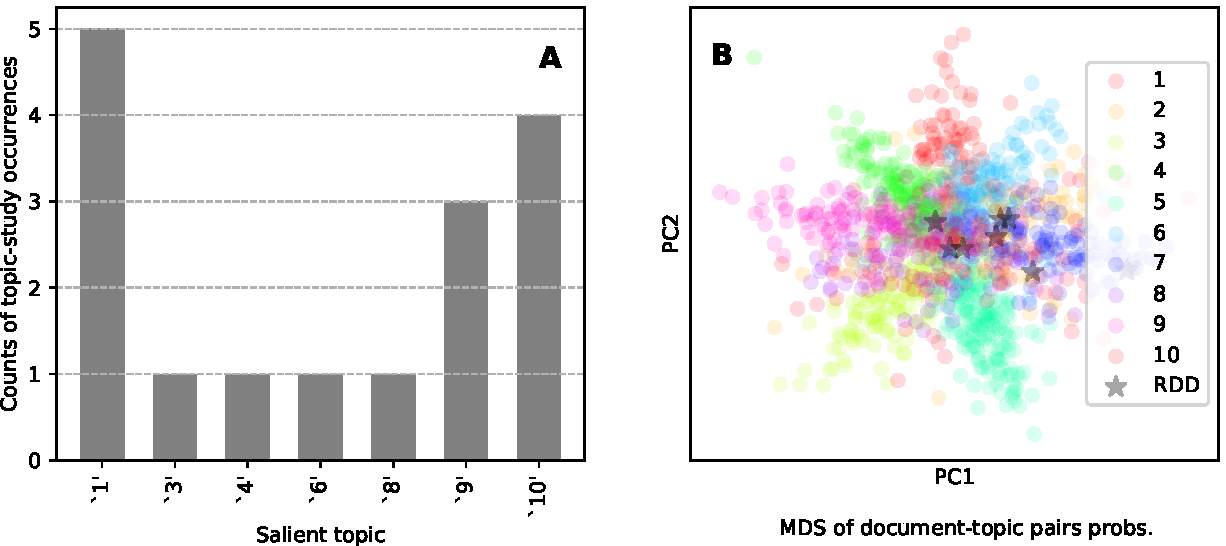
\includegraphics[width=1\textwidth]{_3}
	\label{fig:mds_rdd}
	\caption*{\small\textit{Notes.---} Panel A pictorially depicts the
		information reported in Table~\ref{tab:rdd_list}; Panel B: Data points
		marked with a star denote natural experiments that are folded
		in the topic model trained on the 1,156 articles published in The
		Leadership Quarterly; Topic labels: Topic 1---`female
		leadership'; Topic 2---`emotions and leadership';
		Topic 3---transformational leadership'; Topic 4---`development
		of leadership'; Topic 5---`(neo-)charismatic leadership'; Topic
		6---`cognition and leadership'; Topic 7---`strategic
		leadership'; Topic 8---`ethical leadership'; Topic 9---`nature
		of managerial work'; Topic 10---`leadership
		in teams and decision group.' `MDS' stands for
		multdimensional scaling; `PC1' and `PC2' refer to the
components returned from the MDS analysis.}
\end{figure}


\subsubsection{Regression Discontinuity Design Examples} 

\noindent Our review indicates that to date only a few leadership studies have
used the RD design. We will discuss three studies and analyze their
approach in more detail in order to provide leadership scholars with
insights into applying the RD design for inferring causal relationships.

The first study that we have selected is by Arvate, Galilea and Todescat
(2018). They adopted a sharp RD design to analyze the `queen bee'
phenomenon (Staines, Tavris, \& Jayaratne, 1974), which states that
women in leadership positions do not support---and may even
penalize---female followers. The authors point out that prior studies on
the phenomenon are affected by reverse causality and omitted variable
biases, and, therefore, do not have a causal interpretation. To overcome
these problems, the authors use an RD design focusing on close-run
elections in Brazilian municipalities. Empirical data indicate that
those municipalities in which women are elected as mayors over a male
candidate by a close margin do not differ from municipalities in which
women just lost the election against a male competitor. Thus, near the
threshold (i.e., \(50\%\) of votes), it is almost random as to whether a
woman or a man is assigned to the leadership position. The results do
not provide clear evidence for the queen bee hypothesis. In public
organizations, which are under the influence of mayors, the ratio of
female to male workers is reduced for middle management (anti-women) but
increased for top management (pro-women) in municipalities ruled by
female mayors. Overall, the study applies a sharp RD design to test the
causal effect of female leaders on the career opportunities of female
followers.

The second study is by Heck and Moriyama (2016), who used a sharp RD
design to analyze the indirect relationship between improvement-focused
school leadership and student learning outcomes via school instructional
practices. The authors exploit the discontinuity which results from a
cut-off date for students for starting kindergarten. In the study
setting , students who were 5 years old by December 31 were assigned to
the treatment (i.e., one year further schooling), whereas students who
were 4 years old by December 31 were assigned to the control group
(i.e., one year less schooling). Again, we can argue that near the
cut-off, the student assignment to the treatment and control groups is
as good as random, because parents cannot precisely manipulate the birth
date of their children. Due to students' nesting within schools, the
authors applied a multilevel RD design. The results provide causal
evidence for the benefits of one additional year of schooling (i.e., the
added-year of schooling effect). The authors further show that the
added-year of schooling effect is influenced by the effect of
improvement-focused school leadership on school instructional practices.

Finally, Grönqvist and Lindqvist (2016) used a fuzzy RD design to
analyze how receiving military officer training influences the
probability of attaining a civil leadership position. Directly testing
this relationship is difficult as individuals who receive officer
training differ from individuals who do not receive the training with
regard to observable and unobservable characteristics (e.g., abilities).
To infer the causal effect of the officer training, Grönqvist and
Lindqvist (2016) used discontinuities in test scores as the
identification strategy. That is, all individuals who were drafted in
the Swedish military had to complete a cognitive ability test in which
their abilities were ranked according to four dimensions on a scale from
1 (lowest) to 9 (highest). Although the test score did not determine
whether or not a person received the training, it significantly
increased the probability of being treated. For instance, receiving the
officer training `jumps' from only 2\% of the recruits with a score of
17 to 28 \% for recruits with a score of 18 (Grönqvist \& Lindqvist,
2016). Because of the fuzzy RD design, the authors used two-stage least
squares to estimate the relationship between receiving officer training
and attaining a civil leadership position after the military service.
Their results indicate that officer training clearly influences the
attainment of a civil leadership position. Individuals who received the
officer training have a 75\% higher likelihood of attaining a civil
leadership position compared to the controls. Overall, the study
provides causal evidence for the effectiveness of general leadership
training.

To sum up, the three examples show that both the sharp and the fuzzy RD
designs can provide answers to important questions in leadership
research. The studies were conducted in a variety of contexts (e.g.,
schools, military, public administration) and used very different
assignment variables (e.g., age, voting margins, test scores). However,
all three studies exploited the almost random assignment of units near
the cut-off point for causal inference. 


\section{Natural Experiments in Leadership Research: Guidelines}
\label{sec:guidelines}

\noindent Our review of studies from various leadership-related disciplines,
including economics, business and management, political sciences, and
social sciences, suggests that natural experiments are very effective in
identifying causal relationships. This section provides some guidelines
on further facilitating the use of natural experiments in leadership
research. The key phases of the research design are presented, starting
with the discovery of a natural experiment moving on to the actual form
of the natural experiment, and then finishing with the statistical
analysis. 


\subsection{Discovering Natural Experiments} 

\noindent A major challenge for leadership scholars is to discover natural
experiments. Unlike laboratory and field experiments, researchers cannot
actually design natural experiments. Instead they need to discover
contexts in which a random or as-if random variation has taken place.
Discovering these contexts is difficult. For instance, Dunning (2012, p.
41) argues that discovering natural experiments is `as much art as
science.'

We believe a good way to discover natural experiments is by learning
from prior examples. Firstly, novel research questions can often be
answered by re-using a known/established natural experiment. For
example, the natural experiment of the German reunification has been
exploited to analyze several research questions, such as the impact of
income on health (e.g., Frijters, Haisken-DeNew, \& Shields, 2005), the
transmission of preferences for entrepreneurship from parents to
children (e.g., Wyrwich, 2015), or the legitimation of inequality (e.g.,
Haack \& Sieweke, 2018). Secondly, even when known/established
experiments may not be perfect for addressing a new research question,
by analogical reasoning, researchers can be inspired by such experiments
and discover more appropriate naturally-occurring events for their
research question.

Tables 5, 6, and 7 summarize the research questions, exogenous
variations, and treatments of each individual study included in our
review. Regarding standard natural experiments (see Table 5), many
studies have exploited the introduction of new laws or regulations, such
as a legal reform in Sweden that discontinued the conferral of state
orders of merit (Siming, 2016), or new anti-takeover legislation (Cheng
et al., 2005). Others have used laws that set certain quotas, such as
the proportion of women on the boards of Norwegian firms (Matsa and
Miller, 2013), or that reserved leadership positions for members of
minorities in randomly selected villages (Beaman et al., 2012). Finally,
some studies leverage sudden, exogenous events, such as earthquakes
(Belloc et al., 2016), the successful assassination of political leaders
(Shea and Solis, 2018), or the division of Germany into two states after
1945 (Wyrwich, 2015).

Instrumental variables (see Table 6) can be categorized into four main
groups: i) macro-level variables pertaining to cultural, institutional,
or societal properties, such as the degree of religious piety within a
population (Chintrakarn et al., 2017) or the ratio of voters in favor of
divorce within a region (Amore et al., 2017); ii) random or as-if random
events, such as the gender of a CEO's first born child (Bennedsen et
al., 2007) or the proportion of a firm's founders that are dead (Adams
et al., 2009); iii) spatial distance or related variables, e.g., the
distance of companies from executive recruiting firms (Akyol and Cohen,
2013) or the existence and intensity of one-stop flight connections
between the locations of potential director home addresses and firm
headquarters (Bernile et al., 2018); and finally iv) personal or team
attributes, such as CEO age and tenure (Driver and Coelho Guedes, 2017)
or board size (Kilic and Kuzey, 2016).

Concerning the RD design (see Table 7), the highest number of studies
focus on the margin of victory in an election as an assignment variable
(e.g., Arvate et al., 2018; Boas and Hidalgo, 2011). These studies
exploit the fact that in close elections, the assignment of individuals
to the leader position is almost random.

Ultimately, scholars have discovered natural experiments in a variety of
leadership-related contexts and we recommend leadership scholars to
analyze whether their research questions can be analyzed using the same
natural experiment. Furthermore, leadership scholars may focus on
current or historical institutional changes (e.g., the introduction of
new laws) or try to identify contexts in which assignment to training,
jobs, or ranks are based on or influenced by a unit's score on an
observed variable to identify a new natural experimental context.

\begin{sidewaystable}
	\label{tab:sne_overview}
	\centering	
	\caption{ Standard Natural Experiments---Research Questions, Exogenous
	Variations, and Treatments}
	\resizebox{1\textwidth}{!}{%
        %\begin{tabular}{lllll}
		\begin{tabular}{{@{\extracolsep{1pt}} l >{\quad}p{7cm} p{4cm}
			>{\quad}p{7cm} >{\quad}p{7cm}}}
        \toprule \toprule
        Authors                                      & Research question                                                                                                                                                      & Context                              & Exogenous variation                                                                                                                                                              & Treatment                                                                                                                                                  \\
	\midrule
        Bae \& Yi (2008)               & Do mutual fund managers time the
	market?
	& Equity mutual funds                  & Introduction of the
	``short-short rule'' for mutual funds                                                                                                                          & The short-short rule  hinders mutual fund managers from timing the market                                                                                  \\
        Baekgaard (2011)                             & Whether and how two different organizational leadership models affect the interaction between politicians and administrators                                           & Danish municipalities                & Amalgamation of 232 municipalities into 65 new municipalities                                                                                                                    & Decision to use different administrative leadership models                                                                                                 \\
        Beaman et al. (2012)                         & Does growing up under female leadership raises aspirations and educational attainment for girls?                                                                       & Indian Villages                      & Law that reserves the chief councilor position for women   in a random sample of villages                                                                                        & Female leader                                                                                                                                              \\
	Belloc et al. (2016)            & Do natural catastrophes impact the stability of institutional regimes?                                                                                                     & Medieval Italian cities              & Earthquakes                                                                                                                                                                      & Earthquakes interpreted as manifestation of God's outrage                                                                                                  \\
        Bhavnani (2017)                              & Do the effects of temporary ethnic group quotas persist?                                                                                                               & Indian Villages                      & Quasi-random declaration of reserved seats to be “open” in elections in 1974 and 2008                                                                                            & Discontinuation of ethnic group quotas                                                                                                                     \\
        Breda \& Ly (2015)                          & Does the level of male-domination influence gender bias?                                                                                                               & French higher education              & Examiners in oral examinations are aware of the candidate's gender, whereas examiners are unaware of the gender in written exams                                                 & Proportion of women among professors within a scientific field                                                                                             \\
	Brockman et al. (2015)                   & Does CEO compensation risk influences managers' risk-seeking behavior?                                                                                                 & U.S. public corporations             & Passage of FAS 123R                                                                                                                                                              & Reduction in CEO compensation risk level                                                                                                                   \\
        Byrd et al. (2012)                           & Which governance mechanisms are associated with firm survival and failure?                                                                                             & U.S. firms                           & Thrift crisis of the late 1980s                                                                                                                                                  & Unitary leadership (single CEO/Chairman) vs. dual leadership (two leaders)                                                                                 \\
        Chauchard (2014)                             & Can descriptive representation for a stigmatized group change the beliefs and intentions of members of dominant groups?                                                & Indian villages                      & Discontinuity in the implementation of reservation of political leadership positions for minorities                                                                              & Members of stigmatized groups hold political leadership positions                                                                                          \\
        Chen et al. (2016)                           & Do controlling shareholders hold CEOs accountable to corporate fraud behavior?                                                                                         & Chinese companies                    & Split Share Structure Reform in China                                                                                                                                            & Greater incentive for powerful shareholders to monitor managers                                                                                            \\
	Cheng et al. (2005)                & What value do managers place on the control rights conferred by stock ownership?                                                                                       & U.S. companies                       & Introduction of second-generation anti-takeover legislation                                                                                                                       & Weakening of outsiders' takeover power                                                                                                                     \\
        Cohen \& Wang (2013)                        & Do staggered boards negatively affect firm value?                                                                                                                      & Firms in Delaware                    & Unexpected court rulings in Delaware that affected for a subset of firms the extent to which staggered boards can impede shareholders seeking to replace a majority of directors & Weakening of the anti-takeover force of staggered boards                                                                                                    \\
        Coman (2018)                                 & How does the party affiliation of local elites influence the distribution of central government funds to territorial units?                                            & Romania                             & 2008 Romanian electoral reform                                                                                                                                                   & Change from a closed-list proportional system to a system that requires all members of the parliament to run in single-member districts                    \\
	Cox et al. (2000)             & Does politicians' career goals influence their decision to join a faction?                                                                                             & Japanese bicameral parliament        & Different electoral rules in the two houses of the Japanese parliament                                                                                                           & Lower level of electoral  competition when politicians' join a faction                                                                                     \\
        \bottomrule
	\end{tabular}}
\end{sidewaystable}


\begin{sidewaystable}
	\centering
	\caption*{Cont'd Table 5}
	\resizebox{1\textwidth}{!}{%
        %\begin{tabular}{lllll}
		\begin{tabular}{{@{\extracolsep{1pt}} l >{\quad}p{7cm} p{4cm}
			>{\quad}p{7cm} >{\quad}p{7cm}}}
        \toprule \toprule
                Authors                                      & Research question                                                                                                                                                      & Context                              & Exogenous variation                                                                                                                                                              & Treatment                                                                                                                                                  \\
		\midrule
	Cunat \& Guadalupe (2009)                   & Do deregulation and increased product market competition influence the compensation packages that firms offer to their executives?                                     & U.S. financial sector                & Deregulation laws that reduced entry barriers into the financial sector                                                                                                          & Increased product market competition                                                                                                                       \\
        Dahya \& McConnell (2005)                   & Do boards with
	significant outside directors make different decisions than boards
	dominated by inside directors?
	& U.K. firms                           & Publication of the ``Cadbury
	Report'' which coerced firms into adding outside directors                                                                                            & Appointment of outside directors                                                                                                                           \\
        De Paola \& Scoppa (2015)                   & Is gender discrimination affected by the gender of evaluators?                                                                                                         & Italian universities                 & Random assignment of evaluators                                                                                                                                                  & Degree of committee gender composition                                                                                                                     \\
	De Paola et al. (2010)         & Do gender quotas influence women involvement in political activity?                                                                                                    & Italian local administration         & Some municipalities did not vote under the gender quota regime                                                                                                                   & Gender quotas                                                                                                                                              \\
        Gittell et al. (2008)                        & Does  job design affect the coordination of work?                                                                                                                      & Massachusetts hospital               & Some patients were assigned to hospitalist physicians while others remained under the care of their own private practice physicians                                              & Stage- and site-based specialization                                                                                                                       \\
	Gormley et al. (2013)           & How do boards adjust incentives in response to firms' risk and how do these incentives affect managers' risk-taking?                                                   & U.S. listed corporations             & Workers being exposed to chemicals that have just been found to be toxic                                                                                                         & Increase in left-tail risk (i.e., material risk)                                                                                                           \\
        Guadalupe and Wulf (2010)                    & Does  product market competition influence organizational design?                                                                                                      & large U.S. firms                     & Canada-United States Free Trade Agreement of 1989                                                                                                                                & Increase in competition                                                                                                                                    \\
        Han \& Zhang (2018)                         & What is the net effect of a politically connected board for firms?                                                                                                     & Chinese companies                    & Regulatory change in China                                                                                                                                                       & Bureaucrats were forbidden from sitting on the board of public firms                                                                                       \\
	Hidalgo et al. (2016) & Does auditor appointment affect political accountability?                                                                                                              & Brazilian state audit courts         & Variation in the appointment mechanisms for choosing auditors                                                                                                                    & Auditors insulated from political influence                                                                                                                \\
        Huber \& Arceneaux (2007)                   & Do presidential campaign advertisements mobilize, inform, or persuade citizens?                                                                                        & U.S. presidential elections          & Some individuals living in non-battleground states accidentally received different advertisement because they resided in a media  market adjoining a competitive state.           & High levels or one-sided barrages of campaign advertisements                                                                                               \\
        Jayaraman \& Milbourn (2015)                & Do CEO equity incentives influence financial misreporting?                                                                                                             & U.S. public corporations             & Collapse of Arthur Andersen                                                                                                                                                      & Level of auditor expertise                                                                                                                                 \\
        Jiraporn \& Lee (2018)                      & How do co-opted directors affect dividend policy?                                                                                                                      & U.S. public corporations             & Passage of the Sarbanes–Oxley Act                                                                                                                                                & Increase in board independence                                                                                                                             \\
        Jiraporn et al. (2018)                       & Do independent directors influence corporate innovation?                                                                                                               & U.S. public corporations             & Passage of the Sarbanes–Oxley Act                                                                                                                                                & Increase in board independence                                                                                                                             \\
        Kahn, Li and Zhao (2015)                     & Do shifts in evaluating local officials for promotion affect their efforts to reduce water pollution?                                                                  & Chinese municipalities               & Change in the local political promotion criteria                                                                                                                                 & Higher incentives for local political leaders to reduce border pollution                                                                                   \\
        Knott (2001)                                 & Does hierarchy provide a dynamic advantage?                                                                                                                            & Quick-printing industry              & Establishments leave a franchise system                                                                                                                                          & Establishments lose their hierarchical manager                                                                                                             \\
                                                                       & Having self-employed parents who encountered a great deal of resistance  due to their self-employment                                                      \\
        \bottomrule
	\end{tabular}}
\end{sidewaystable}

\begin{sidewaystable}
	\centering
	\caption*{Cont'd Table 5}
	\resizebox{1\textwidth}{!}{%
        %\begin{tabular}{lllll}
		\begin{tabular}{{@{\extracolsep{1pt}} l >{\quad}p{7cm} p{4cm}
			>{\quad}p{7cm} >{\quad}p{7cm}}}
        \toprule \toprule
               Authors                                      & Research question                                                                                                                                                      & Context                              & Exogenous variation                                                                                                                                                              & Treatment                                                                                                                                                  \\
\midrule
	       Laustsen and Petersen (2017)                 & Are political candidates and leaders with dominant, masculine physical features  more preferred under conditions of conflict than of cooperation?                      & Poland and Ukraine                   & Crimea crisis in 2014                                                                                                                                                            & Condition of conflict                                                                                                                                      \\
        Matsa \& Miller (2013)                      & Does female leadership affect corporate decision making?                                                                                                               & Norwegian listed firms               & Law that sets a quota for women in the board of directors                                                                                                                        & Increase of female leaders                                                                                                                                 \\
        Poulos (2019)                                & Does personal wealth cause individuals to select into public office?                                                                                                   & Georgia                              & 1805 and 1807 Georgia land lotteries                                                                                                                                             & Increase in wealth due to lottery                                                                                                                          \\
        Rickman \& Witt (2008)                      & Do principals who exercise favouritism towards certain agents harm other agents?                                                                                       & English soccer                       & Introduction of professional referees to the English Premier League                                                                                                              & A group of referees was retained for the whole soccer season on a full salary                                                                              \\
        Shea and Solis (2018)                        & Does leader tenure influence country's creditworthiness?                                                                                                               & Cross-country analysis               & Successful executive assassination                                                                                                                                               & Leader death                                                                                                                                               \\
        Siming (2016)                                & Do orders of merit function as an external form of perquisite through which the government can supplement the compensation given by a publicly listed firm to the CEO? & Swedish companies                    & 1974 legal reform in Sweden                                                                                                                                                      & Discontinuing the conferral of orders of merit to citizens                                                                                                 \\
	Tabvuma et al. (2014)              & Does change in political leadership influence job satisfaction in the public sector?                                                                                   & British public sector                & Change in the political party which is governing at the national level                                                                                                           & The ruling political party matches the political preference of the public sector employee                                                                  \\
       Tosun (2016)                                 & Do CEO option compensation changes influence firm leverage changes?                                                                                                    & U.S. public corporations             & Internal Revenue Code 162(m) tax law                                                                                                                                             & Increased option compensation for CEOs                                                                                                                     \\
        Valdini (2012)                               & Do  electoral systems affect candidate selection, especially female political leaders?                                                                                 & Elections in Japan                   & Electoral reforms of the Japanese House of Representatives in 1994                                                                                                               & Move towards a greater orientation towards issues and parties                                                                                              \\
        Vo \& Canil (2019)                          & Is CEO pay disparity due to efficient contracting or CEO power?                                                                                                        & U.S. public corporations             & Introduction of FASB ASC 718 in 2005                                                                                                                                             & All accounting benefits associated with option grants were removed                                                                                         \\
        Wyrwich (2015)                               & Do parents transmit  preferences for entrepreneurship to their children?                                                                                               & Entrepreneurs in Germany             & German divide in 1945 which leads to some parents of entrepreneurs growing up in a socialist country                                                                             & Having self-employed parents who encountered a great deal of resistance  due to their self-employment                                                      \\
        \bottomrule
	\end{tabular}}
\end{sidewaystable}


\begin{sidewaystable}
	\centering
	\label{tab:iv_overview}
	\caption{Instrumental Variable Designs---Research Questions, Exogensous
		Variations, and Treatments}
	\resizebox{1\textwidth}{!}{%
        %\begin{tabular}{lllll}
		\begin{tabular}{{@{\extracolsep{1pt}} l >{\quad}p{7cm} p{4cm}
			>{\quad}p{7cm} >{\quad}p{7cm}}}
        \toprule \toprule
        Authors                                      & Research question                                                                                                                                                      & Context                              & Exogenous variation                                                                                                                                                              & Treatment                                                                                                                                                  \\
	\midrule
Adams et al. (2009)                    & Do founder-CEOs influence firm performance?                                                                               & Family firms                                                      & (1) proportion of the firm's founders that are dead; (2) number of people who founded the company                                                                                               & Founder-CEO                                                                   \\
Adhikari (2018)                        & Do firms led by female top executives hold more cash?                                                                     & U.S. listed companies                                             & Fraction of registered men between the ages of 18 and 44 who were drafted or enlisted for WWII in a state                                                                                       & Number of female executives                                                   \\
Adkins et al. (2007)                   & Do managerial compensation and ownership influence the use of foreign‐exchange derivatives by U.S. bank holding companies & Large bank holding companies                                      & (1) number of employees, (2) number of subsidiaries; (3) number of offices; (4) CEO age; (5) 12 month maturity mismatch; (6) market-to-book ratio; (7) foreign interest income dummy            & Managerial compensation and ownership                                         \\
Aghion et al. (2013)                   & Does institutional ownership influence firm innovation?                                                                   & S\&P 500 firms                                                    & Firms’ addition to the S\&P 500 index                                                                                                                                                           & Institutional ownership                                                       \\
Akyol \& Cohen (2013)                 & Does the use of executive search firms for board member search influence corporate governance?                            & U.S. public corporations                                          & Geographic distance of companies to executive search firms                                                                                                                                      & Use of executive search firms                                                 \\
Amore et al. (2017)                    & Does leadership by couples affect the profitability of family firms?                                                      & Italian family firms                                              & Regional ratio of voters in favor of divorce                                                                                                                                                    & Leadership by couples                                                         \\
Amore et al. (2014)                    & Do gender interactions at the top of the corporate hierarchy affect firm performance?                                     & Italian family firms                                              & (1) gender composition of the pool of potential family heirs; (2) geographic variations in gender stereotypes                                                                                   & Gender interactions                                                           \\
Arora (2018)                           & Does the effort of financially linked independent directors enable firms to reemerge from bankruptcy?                     & U.S. firms                                                        & (1) Board meeting fees; (2) prime interest rate movement; (3) board size                                                                                                                        & Effort of financially linked independent  directors                           \\
Artz et al. (2017)                     & Does the competence of supervisors influence the quality of employees’ lives?                                             & US and UK employees                                               & (1) whether the supervisor has a college degree; (2) whether the supervisor worked his or her way up in the organization                                                                        & Supervisor competence                                                         \\
Azoulay et al. (2017)                  & Do young scientists adopt their advisers’ orientations toward commercial science?                                         & Academics from the U.S.                                           & (1) proximity between scholars’ undergraduate institutions and the universities where they might become postdoctoral fellows; (2) shared nationality between the scholar and a potential mentor & Social matching                                                               \\
Barros (2007)                          & Which factors influence pay and performance of CEOs?                                                                      & Portuguese non-profit organizations                               & (1) number of stockholders in the company; (2) father's education                                                                                                                               & Board composition                                                             \\
Bennedsen et al. (2007)                & Does the appointment of family CEOs negatively affect firm performance?                                                   & Danish family firms                                               & Gender of CEO's first born child                                                                                                                                                                & Hiring of an external CEO                                                     \\
Bernile et al. (2018)     & Does board diversity influence corporate policies and risk?                                                               & North American listed companies                                   & Existence and intensity of one-stop flight connections between the locations of potential director home addresses and firm headquarters                                                         & Board diversity                                                               \\
Chen et al. (2017)         & Does gender diversity in boardrooms influence dividend payouts?                                                           & S\&P 1500                                                         & (1) fraction of male directors linked to female directors; (2) female-to-male labor force participation ratio                                                                                   & Board gender diversity                                                        \\

	\bottomrule
	\end{tabular}}
\end{sidewaystable}


\begin{sidewaystable}
	\centering
	\caption*{Cont'd Table 6}
	\resizebox{1\textwidth}{!}{%
        %\begin{tabular}{lllll}
		\begin{tabular}{{@{\extracolsep{1pt}} l >{\quad}p{7cm} p{4cm}
			>{\quad}p{7cm} >{\quad}p{7cm}}}
        \toprule \toprule
        Authors                                      & Research question                                                                                                                                                      & Context                              & Exogenous variation                                                                                                                                                              & Treatment                                                                                                                                                  \\
	\midrule
Chintrakarn et al. (2017)              & Does religious piety substitute for corporate governance?                                                                 & U.S. firms                                                        & degree of religious piety in the past in the population surrounding a corporate headquarter                                                                                                     & Current religious piety in the population surrounding a corporate headquarter \\
	Conroy \& Weiler (2016)               & Does female ownership influence firm performance?                                                                         & U.S. startups                                                     & (1) change in divorce rate; (2) growth in female labor force participation                                                                                                                      & Female owner                                                                  \\
Conyon \& He (2017)                   & Does gender diversity in boardrooms influence firm performance?                                                           & US firms                                                          & Percentage of female residents in the US state where the given company has its headquarter                                                                                                      & Board gender diversity                                                        \\
Dal Bó et al. (2009)       & Why do political dynasties persist?                                                                                       & U.S. congress                                                     & Successful first reelection attempt                                                                                                                                                             & Long tenure in power                                                          \\
Dasgupta (2018)                        & Does technological change contribute to political turnover?                                                               & Indian agriculture                                                & Share of district land with a naturally occurring aquifer interacted with a dummy variable that “switches on”’ for all districts with the introduction of HYV crops                             & Technological change                                                          \\
Delis et al. (2017)                    & Do board members from countries with different genetic diversity levels influence corporate performance?                  & North American and U.K. listed companies                          & (1) migratory distance from East Africa; (2) the level of ultraviolet exposure in the directors’ country of nationality                                                                         & Genetic diversity within a country                                            \\
Driver \& Coelho Guedes (2017)        & Is R\&D expenditure reduced in cases of imminent departure of the CEO?                                                    & UK service and manufacturing firms                                & (1) CEO age; (2) CEO tenure; (3) profit shock                                                                                                                                                   & CEO departure                                                                 \\
Frantz \& Stein (2017)                & Do institutionalized leadership succession rules influence the likelihood that dictators confront coups?                  & Dictatorships                                                     & A regime took power at independence                                                                                                                                                             & Institutionalized leadership succession rules                                 \\
Gabel \& Scheve (2007)                & To what extent does elite opinion about policy shape public opinion?                                                      & European countries                                                & Change in electoral laws                                                                                                                                                                        & Elite polarization                                                            \\
Harjoto \& Rossi (2019)               & Do religiosity and female representation on the board influence corporate social responsibility?                          & Italian listed companies                                          & (1) number of words in the encyclicals and other writings that are related to “religiosity”; (2) number of words in the encyclicals that are related to gender diversity                        & Religiosity in the population and women  on the board of directors            \\
Hearn and Filatochev (2019)            & Does private equity ownership influence the probability of the founder's retention as CEO?                                & IPOs in emerging markets                                          & Numbers of private equity investors                                                                                                                                                             & Private equity ownership                                                      \\
Hooghiemstra, Kuang and Qin (2017)     & Does ‘readability’ of a remuneration report influence the level of shareholder say-on-pay voting?                         & UK-listed firms                                                   & Readability of CEO letter                                                                                                                                                                       & Readability of remuneration report                                            \\
Izgi \& Akkas (2012)                  & Does top management gender diversity influence firm performance?                                                          & Turkish firms                                                     & (1) CEO MBA; (2) Big 4 Audit                                                                                                                                                                    & Female CEO                                                                    \\
Khwaja (2009)                          & Can project design compensate for  community-specific constraints in social capital?                                      & Community-maintained infrastructure projects in Northern Pakistan & Characteristics of hereditary leader households (e.g., does the leader household has a young and healthy male member?)                                                                          & Having a project leader                                                       \\
Kilic \& Kuzey (2016)                 & Does gender diversity in boardrooms improve firms’ economic performance?                                                  & Turkish listed companies                                          & (1) board size; (2) board independence; (3) firm size; (4) leverage                                                                                                                             & Board gender diversity                                                        \\
Li et al. (2018)                       & Does superior environmental, social and corporate governance disclosure affect firm value?                                & FTSE 350 firms                                                    & Firm-level initial value of the ESG disclosure score                                                                                                                                            & Environmental, social and corporate governance disclosure                     \\
Lin et al. (2011)                      & Do managerial incentives and CEO characteristics influence a firm’s innovation activities?                                & Chinese manufacturing firms                                       & Industry-location averages                                                                                                                                                                      & Provision of managerial incentive schemes                                     \\
	\bottomrule
	\end{tabular}}
	\label{tab:discover_tr_iv_2}
\end{sidewaystable}


\begin{sidewaystable}
	\centering
	\caption*{Cont' Table 6}
	\resizebox{1\textwidth}{!}{%
        %\begin{tabular}{lllll}
		\begin{tabular}{{@{\extracolsep{1pt}} l >{\quad}p{7cm} p{4cm}
			>{\quad}p{7cm} >{\quad}p{7cm}}}
        \toprule \toprule
        Authors                                      & Research question                                                                                                                                                      & Context                              & Exogenous variation                                                                                                                                                              & Treatment                                                                                                                                                  \\
	\midrule
Markussen \& Roed (2017)              & Do gendered peer influences affect early career entrepreneurship?                                                         & Norwegian entrepreneurs                                           & Entrepreneurship activity among the schoolmates’ parents                                                                                                                                        & Peer influences                                                               \\
Nicolosi and Yore (2015)               & Does a CEO's marital status  influence their firm's investment and compensation policies                                  & S\&P 1500                                                         & Religious CEO                                                                                                                                                                                   & CEO marital status                                                            \\
Pascal et al. (2017)       & Does a CEO's business education influence the financial and social performance of microfinance institutions?              & Global microfinance institutions                                  & Microfinance institution age                                                                                                                                                                    & CEO business education                                                        \\
Rouse (2012)                           & Does high school leadership affect subsequent educational attainment?                                                     & U.S. high schools                                                 & (1) school‐level measure of leadership opportunities; (2) oldest child in the family                                                                                                            & High school leadership                                                        \\
Sabatier (2015)                        & Does gender diversity in boardrooms improve firms’ economic performance?                                                  & French publicly listed companies                                  & Average ratio of women in connected boardrooms                                                                                                                                                  & Board gender diversity                                                        \\
Shue \& Townsend (2019)               & Does an increase in stock option grants affect CEO risk‐taking?                                                           & North American listed companies                                   & (1) whether each CEO‐year is predicted to be the first year of a new fixed‐value cycle; (2) variation in the value of options granted within fixed‐number and fixed‐value cycles                & Increase in stock option grants                                               \\
Sun \& Hovey (2013)                   & Does executive compensation influence management discretionary behavior over financial reporting?                         & Australian Securities  Exchange (ASX)   listed  companies         & Median value of discretionary accruals for a portfolio of firms                                                                                                                                 & Executive compensation                                                        \\
Vries (2012)                           & Does personality influence leadership styles?                                                                             & Large municipality organization                                   & Different-source personality ratings                                                                                                                                                            & Leader personality                                                            \\
Wu (2015)                              & Does inequality influence trade openness in authoritarian regimes?                                                        & Authoritarian regimes                                             & Ratio between two age groups                                                                                                                                                                    & Income inequality                                                             \\
Yang et  al. (2019)           & Do networks influence persons' placement into leadership positions of varying levels of authority                         & MBA programme                                                     & degree of expose to  same-gender classmates from other home sections                                                                                                                            & Composition of students' inner circle                                         \\
	\bottomrule
	\end{tabular}}
	\label{tab:discover_tr_iv_3}
\end{sidewaystable}


\begin{sidewaystable}
	\centering
	\label{tab:rdd_overview}
	\caption{Regression Discontinuity Designs---Research Questions,
	Exogensous Variations, and Treatments}
	\resizebox{1\textwidth}{!}{%
        %\begin{tabular}{lllll}
		\begin{tabular}{{@{\extracolsep{1pt}} l >{\quad}p{7cm} p{4cm}
			>{\quad}p{7cm} >{\quad}p{7cm}}}
        \toprule \toprule
        Authors                                      & Research question                                                                                                                                                      & Context                              & Exogenous variation                                                                                                                                                              & Treatment                                                                                                                                                  \\
	\midrule
	Arvate et al. (2018)        & Do female leaders harm the career of female followers?                                                                              & Mayoral elections in Brazil & Margin of victory in election                                                 & Female leader                                           \\
Boas \& Hidalgo (2011)             & Does incumbency influence politicians’ ability to control the media and does media control affect their future electoral prospects? & Elections in Brazil         & Margin of victory in election                                                 & Incumbency                                              \\
Butler (2009)                       & Does the incumbency advantage enjoyed by freshmen differ from the incumbency advantage enjoyed by non-freshmen incumbents?          & U.S. house elections        & Margin of victory in previous election                                        & Incumbency                                              \\
Dal Bó et al.    (2009)    & Why do political dynasties persist?                                                                                                 & U.S. congress elections     & Margin of victory in election                                                 & Long tenure in power                                    \\
Dunning \& Nilekani (2013)         & Do ethnic quotas induce distribution of material benefits to members of disadvantaged groups?                                       & Elections in India          & Proportion of the local population comprised of marginalized castes or tribes & Reserved seats in the council for members of minorities \\
Grönqvist and Lindqvist (2016)      & Does training during the Swedish military service influence the probability of attaining a civil leadership position?               & Swedish army                & Score on a cognitive ability test                                             & Received military officer training                      \\
Heck \& Moriyama (2010)            & Does school leadership influence students' educational performance?                                                                 & School                      & Student age                                                                   & Additional year of schooling                            \\
Lechler \& McNamee (2018)          & Does colonial rule influence support for democracy?                                                                                 & Namibia                     & Location of the Police Zone boundary                                          & Form of colonial rule                                   \\
	\bottomrule
	\end{tabular}}
\end{sidewaystable}


\subsection{Deciding about the Form of the Natural Experiment}

\noindent Once an exogenous, naturally-occurring variation has been discovered,
scholars need to decide the form of natural experiment to adopt. This choice is
key to a design's internal validity as standard natural experiments, IV, and RD
designs build on specific assumptions about the mechanisms that are presumed to
generate the observed data (Dunning, 2012; Imbens \& Wooldridge, 2009). Our
decision tree (Figure~\ref{fig:decision_tree}) is designed to help scholars
select the most suitable research design.

\begin{figure}[!htbpp]
	\centering
	\caption{Decision Tree Linking Treatment Attributes, Assumptions, and
	Forms of Natural Experiments}
	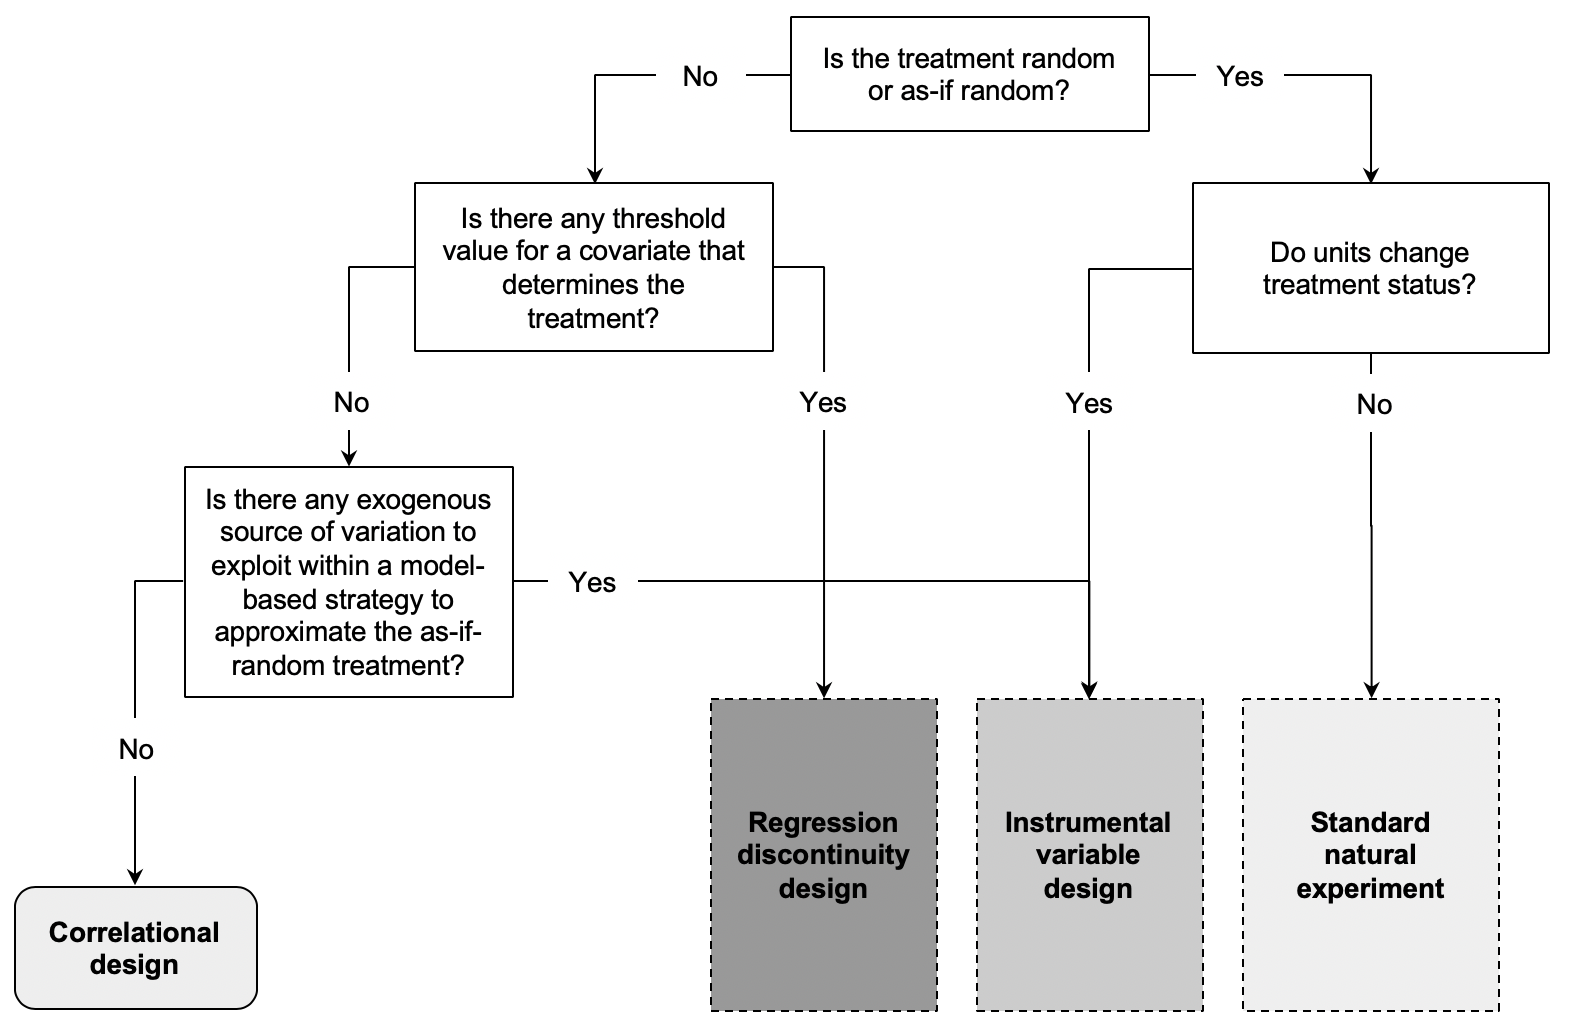
\includegraphics[width=1\textwidth]{_7}
	\label{fig:decision_tree}
\end{figure}

The first question leadership scholars need to answer concerns the
assignment process: is the assignment of units to the treatment truly
random, `as-if random' (i.e., the assignment process resembles a true
randomization, Dunning, 2012), or non-random? Although a true
randomization is a hallmark of laboratory and field experiments
(Podsakoff \& Podsakoff, 2019), it is seldom found in natural
experiments---except for studies that use lotteries (e.g., Angrist,
1990).

In fact, most natural experiments are characterized by an as-if random
assignment. The as-if random assignment poses some challenges for
leadership scholars, because they need to evaluate the quality of the
as-if randomization; that is, the extent to which it is plausible to
assume that the assignment process (closely) resembles a true
randomization. Dunning (2012) recommends assessing the quality of the
as-if randomization based on three criteria. First, researchers should
investigate whether units had \emph{information} that they would or
would not receive the treatment. Second, researchers need to check
whether units had \emph{incentives} to self-select into the treatment
group or control group . Third, researchers should analyze whether not
only units had incentives but also \emph{capacity} to self-select into a
treatment status. For the assessment, Dunning (2012) suggests using both
qualitative evidence (e.g., documents, interviews) and quantitative
evidence (e.g., balance tests).

Jones and Olken (2005), for example, jointly used qualitative and
quantitative evidence to evaluate the plausibility of as-if
randomization. They used qualitative evidence, such as leaders'
biographies, to determine whether the nature of death of political
leaders was truly exogenous (e.g., due to health issues or accidents).
At the same time, they provide quantitative evidence, such as the result
of a logistic regression, to back up the assumption that economic
conditions do not predict the death of political leaders.

If the assignment process is random or as-if random, then researchers
need to check the second question: are units allowed to change their
treatment status, moving from the treatment (control) to the control
(treatment) group? This check is important, because units that comply
with the assignment (`compliers') probably differ from units that do not
comply with the assignment (`non-compliers'). For instance, in Angrist's
(1990) study on the effect of military service on lifetime earnings,
subjects were assigned to the treatment (military service) and control
group (no military service) based on their date of birth and the result
of a draft lottery. However, some subjects who were eligible based on
the result of the lottery did not serve in the military, because they
went to college or moved outside the U.S. We can assume that these
non-compliers differ from the compliers (i.e., those citizens who were
eligible and did serve and those who were not eligible and did not serve
in the military) regarding knowledge, values, attitudes etc., and that
these differences are probably correlated with their lifetime earnings.
Therefore, leadership scholars should, if possible, focus on the
compliers in their analysis (Dunning, 2012) or should try to estimate
the ratio of compliers within a population (see, e.g., Angrist, 1990).

If researchers answer the first question positively (i.e., random or
as-if random assignment) while negatively answering the second one
(i.e., change of treatment status), then the natural experiment at hand
represents a standard natural experiment, whose data can be analyzed
either using Neyman's potential outcome framework or by adopting
model-based adjustments (we discuss the analysis in more detail below).
If both answers are positive, then the natural experiment is an IV
design.

If the assignment to the treatment is neither random nor as-if random,
then leadership researchers need to check whether a unit's score on an
observed variable influences the assignment. An assignment based on a
unit's score on a covariate is a hallmark of the RD design. The
assignment may take two forms (Lee \& Lemieux, 2010). First, in the
sharp RD design, a unit's score on a covariate \emph{determines} the
assignment. For instance, in the study by Arvate and colleagues (2018),
the assignment of women to political leadership positions was determined
by their share of votes in mayoral elections. Second, in the fuzzy RD
design, a unit's score on a covariate affects the \emph{probability} of
receiving the treatment. For instance, in Grönqvist and Lindqvist's
(2016) study, a person's score on a cognitive test influenced the
probability of receiving leadership training.

Finally, if the assignment to the treatment is not based on a unit's
score on an observed variable, then leadership researchers need to
determine whether they exploit an exogenous source of variation that
they can use to approximate an as-if random treatment. If they answer
'yes' to the questions, then this exogenous source of variation
represents an instrument and the natural experiment can be classified as
an IV design. For instance, in the study by Bennedsen and colleagues
(2007), the hiring of a family CEO versus an external CEO is neither
random nor as-if random. However, the authors use an exogenous source of
variation---the gender of the firstborn child as an instrument to
estimate the causal effect of hiring professional managers on firm
performance. If researchers cannot exploit such an exogenous source of
variation, then their context represents a correlational design, which
does not support causal inference.


\subsection{Analyzing Natural Experiments}

\noindent After leadership scholars have determined the form of the natural
experiment, they need to analyze the experiment. Although the different
forms may require different types of data analysis, simplicity and
transparency are the underlying factors (Dunning, 2012). Simplicity
means that leadership scholars do not necessarily need to apply complex
statistical techniques to analyze natural experiment data. A simple
difference-of-means or difference-of-proportions test is often
sufficient to estimate the average causal effect of the treatment.
Simplicity in data analysis also generally implies greater transparency.
For instance, difference-of-means or difference-of-percentages tests
provide a more transparent estimate of the average causal effect than
multivariate regression models that contain several covariates. Although
researchers cannot always follow these principles due to the specific
circumstances of a natural experiment and they need to use model-based
adjustments, such as including covariates or adjusting standard errors,
we believe that they should consider the general principles and prefer
`simpler' models over more complex ones.

\subsubsection{Analyzing Standard Natural Experiments}

\noindent \textbf{Estimation of the Average Causal Effect in the Standard Natural
Experiment.} The analysis of standard natural experiments is reasonably simple. Since
the assignment of units to the treatment is random or as-if random, it
is possible to infer a causal effect within Neyman's potential outcome
framework (also called the Neyman-Rubin model; see Rubin, 2005).
Neyman's framework is both simple and transparent (Dunning, 2012).
Scholars may want to use the difference-of-means or
difference-of-proportion tests that are widely applied in laboratory
experiments. Therefore, either a t-test (for smaller sample sizes) or
z-test (for larger sample sizes, see Dunning, 2012) could suffice to
conduct causal research with observational data.

Alternatively, a regression-based approach could be desirable when
qualitative evidence and/or institutional knowledge on the part of the
researchers indicate the treatment may not be random or as-if random.
Such an analytical strategy would enable a comparison between the
findings from the difference-of-means or difference-of-percentages test
with the estimates obtained through a multivariate regression containing
the covariates that are presumed to correlate with the treatment. In the
regression-based approach, the population regression function is:

\begin{equation}\label{eq:sne_equation}
	y = \beta X + \gamma t + \lambda D + \delta t D + u
\end{equation}

In Equation~\ref{eq:sne_equation}, $\beta$ represents the coefficient for a
vector of covariates $X$; $\gamma$ represents the coefficient for the time
trend common for treatment and control group; $\lambda$ represents the
systematic difference in the outcome across the treated and the control cases
(group-specific time-invariant difference); and $\delta$ represents the
coefficient for the interaction of the group and time variable, which estimates
the average causal effect of the treatment on the outcome $y$; and $u$
represents the error term (Imbens \& Wooldridge, 2009).

\noindent \textbf{Plausibility of the Assumptions of the Standard Natural Experiment.}
The analysis of the standard natural experiment using the Neyman
framework builds on two assumptions. First, units are randomly or as-if
randomly assigned to the treatment. In order to provide evidence of the
quality of the (as-if) randomization, Dunning (2012) recommends
conducting balance tests. Currently, many researchers use
mean-difference tests (t-tests) to analyze variations between units in
the treatment and control group along relevant pre-treatment covariates.
However, this approach is sensitive to the sample size, i.e., even small
differences become statistically significant if the sample size is
large. To reduce this problem, scholars can use normalized differences,
which are unaffected by sample size (for a detailed discussion of how to
calculate the normalized differences, see Imbens \& Wooldridge, 2009). A
further disadvantage of mean-difference tests is that it is difficult to
determine whether the control and treatment groups are balanced. For
instance, if researchers conduct t-tests for 20 covariates, we would
expect to find at least one statistically significant difference simply
as the result of chance. Therefore, we suggest conducting joint
hypothesis tests, for example by regressing the binary treatment
variable on the covariates and using a $\chi^{2}$ test to
analyze whether the coefficient of the covariates differs from zero
(McKenzie, 2015).

Second, the Neyman framework builds on the assumption that the outcomes
of a unit are only influenced by the unit's treatment-assignment status.
This assumption is also called the noninterference assumption or the
``stable unit treatment value assumption (SUTVA)'' (Imbens \& Rubin,
2015). SUTVA refers to a situation in which the treatment status of
other units affects a unit's outcome. For instance, a company aims to
analyze whether leadership training increases the effectiveness of their
leaders. For this reason, the company assigns some leaders to a
leadership training programme (treatment group), whereas other leaders
receive no training (control group). However, because leaders work
together within the same company and interact with each other, leaders
in the treatment group may share some of the knowledge they learned in
the training programme with leaders in the control group. This spillover
violates the SUTVA and leads to an underestimated average causal effect
(Morgan \& Winship, 2015). Unfortunately, there is currently no clear
solution to SUTVA violations, though Belloc et al. (2018) used corrected
standard errors to deal with such possible violations, and Selb and
Munzert (2018) excluded units in the control group which were in close
spatial proximity to treated units, because these units were
particularly likely to be treated by accident.

Since there is no `solution' to the SUTVA violation, we recommend that
(i) both the statistically adjusted and unadjusted estimation results
are reported, as this may provide insights into the extent to which a
possible SUTVA violation affects the results, and (ii) the role of
social interactions needs to be to explicitly taken into account, which
could reveal important boundary conditions for the effect under
examination (see Sinclair, 2011).

\noindent \textbf{Testing the Robustness of the Results of the Standard Natural
Experiment.} There are several options to test the robustness of the results of a
standard natural experiment. Firstly, the results can be tested for
robustness if they include pre-treatment covariates in the analysis. For
instance, Beaman and colleagues (2012) showed the results of both
difference-in-means tests and ordinary least squares coefficients
adjusted for covariates despite random assignment of women to a
leadership position. Although the inclusion of covariates is unlikely to
have a high impact on the average causal effect in a natural experiment
with high plausibility of as-if random assignment, adding
covariates---especially those that are unbalanced between the treatment
and control group---increases the transparency and credibility of the
results in the eyes of other researchers. Therefore, the best approach
is to estimate the average causal effect with and without covariates and
if there are significant differences then potential reasons for these
differences should be explored in more detail.

Secondly, if the passing of a new law, regulation or quota is at the
basis of the experiment, then Matsa and Miller's (2013) approach should
be followed, i.e., by conducting additional tests for different types of
units---e.g., units that almost complied with a quota or law before the
inception, and units that had a large distance from compliance. Matsa
and Miller argue that they would expect greater effects for firms with a
greater distance from compliance with the gender quota than for firms
that almost complied with the quota. Such an additional test is
important because it can provide further evidence that the observed
effect is caused by the new law, regulation, or quota and not by an
unrecognized event that affected the units in the treatment group.

Thirdly, Matsa and Miller's (2013) also use matching
methods (e.g., propensity score matching). Matching methods should be
used if units in the treatment and control group differ from each other
with regard to several (observable) covariates. The covariates can be
used to match treated units with control units that are highly similar
with regard to the observed covariates. Although matching methods are no
replacement for an as-if randomization, because they do not ensure that
units in the treatment and control groups do not differ with regard to
observed \emph{and} unobserved covariates, these methods can provide
further insights into the robustness of the initial results.

\subsubsection{Analyzing Instrumental Variable Designs}

\paragraph{Estimation of the Average Causal Effect in the IV
Design.}

In the IV design (see Figure~\ref{fig:iv_path}), we estimate the causal effect
of an endogenous treatment variable $D$ by identifying an instrument $z$ that
affects $D$ but is otherwise unrelated to the outcome $y$ (Abadie \& Cattaneo,
2018). The key idea of the IV design is that we only retain the variation in
the treatment that is caused by an exogenous variation in the instrument, while
ruling out the association between the treatment and possible covariates $A$
and $B$ (see Figure~\ref{fig:iv_path}). For instance, in hist study on  the
effects of military service on future earnings, Angrist (1990) isolates
the variation in the treatment (i.e., military service) that was
caused by an exogenous variation (i.e., Vietnam draft lottery) of the
instrument (i.e., eligibility of being drafted for military service).

The Wald estimator is the simplest and most transparent way to estimate the average causal
effect in the IV design (Dunning, 2012):

\begin{equation}
	\rho = \frac{E[Y_{i} | Z_{i} = 1] - E[Y_{i} | Z_{i} = 0]}
	{E[D_{i} | Z_{i} = 1] - E[D_{i} | Z_{i} = 0]}
        \label{eq:iv_equation}
\end{equation}

The IV estimate $\rho$ in Equation~\ref{eq:iv_equation} equals the difference
in the outcome variable between treated $E[Y_{i} | Z_{i} = 1]$ and $E[Y_{i} |
Z_{i} = 1]$ controls divided by the ratio between treated $E[D_{i} | Z_{i} =
1]$ and controls $E[D_{i} | Z_{i} = 1]$. Such an equation provides some first
insights into the IV estimate $\rho$.

While the Wald estimator should be applied for estimations with a single
instrument without any covariates, researchers recommend using the
two-staged least squares (2SLS) estimator for multiple instruments or
when covariates are added (Angrist \& Pischke, 2009). In the latter
case, we use two steps to estimate the causal effect of the treatment.
In the first-stage (equation 3), we regress the treatment variable $D$
on a vector of covariates $X$ and on the exogenous instrument $Z$:

\begin{equation}
	D = \gamma_{1} X + \gamma_{2} Z + v 
	\label{eq:iv_first_stage}
\end{equation}

In the second-stage Equation~\ref{eq:iv_second_stage}, we regress the outcome
variable (Y) on the covariates (X) and predicted values of the treatment from
the first-stage regression: 

\begin{equation}
	y = \beta_{1} X + \beta_{2} \widehat{D} + u
	\label{eq:iv_second_stage}
\end{equation}

\noindent where $\beta_{2}$ denotes the average causal effect
of the treatment.

\noindent \textbf{Evaluation of the Plausibility  of the Assumptions of the IV
Design.} The IV design relies on several assumptions. In line with Angrist \&
Pischke (2009), we emphasize the following elements: (i) exogeneity of
the instrument; (ii) relevance of the instrument; and (iii) the
exclusion restriction.\footnote{Please note that assumption (i) and
  (iii) are often combined. In the interest of clarity, we follow
  Angrist and Pischke (2009) and separately consider each assumption.}
The first assumption---exogeneity of the instrument---means that the
instrument is uncorrelated with the error term \(u\), included in
Equation~4 . In other words, the instrument is assumed not to be related
to the causes of the dependent variable (Sovey \& Green, 2011). Arguing
this assumption is consistent with a target population regression
function, and the dataset at hand is particularly problematic. In fact,
it is not possible to empirically test the exogeneity of an instrument
(Wooldridge, 2009). Furthermore, recent simulation studies indicate that
endogenous instruments produce causal effect estimates ``that are
inferior to those reported by OLS regression'' (Semadeni et al., 2014,
p. 1071). These concerns become less accentuated when units are randomly
assigned to the instrument (Dunning, 2012), as in the case of lotteries
(Angrist, 1990). Even if the assignment is not truly random, one can
still argue for the exogeneity of the instrument. For instance,
Bennedsen and colleagues (2007) point out that their instrument---the
gender of the firstborn child---is as-if random and they expand on
qualitative evidence by observing that technologies to identify the
child's gender before the birth were not widespread at the time, so that
abortion due to the child's gender was unlikely. These arguments provide
convincing evidence for the exogeneity of the instrument, despite the
lack of a direct test.

The second assumption---the relevance of the instrument---implies that
\(Z\) and \(D\) are correlated. Specifically, instruments can be
categorized into weak, moderate and strong according to the magnitude of
the \(Z - D\) correlation. In order to assess an instrument's strength,
the canonical test can be used which is based on the F-statistic of the
first-stage regression (Semadeni et al., 2014).\footnote{Interested
  readers find an overview of critical values for the weak instrument
  test in Stock and Yogo (2005).} Exploiting the canonical test, Olea
and Pflueger (2013) developed a weak-instrument test, which is robust to
heteroscedasticity, autocorrelation, and clustering, and which is more
efficient than the standard Stock and Yogo (2005) test. Strong
instruments should be the norm in the IV design, because weak and
moderate instruments lead to inflated standard errors, although the
estimated regression slopes are unbiased (Semadeni et al., 2014).

The third assumption---exclusion restriction---means that \(Z\) has no
influence on \(y\) apart from the effect that is conveyed through \(D\)
(Sovey \& Green, 2011). Similarly to the exogeneity assumption, the
exclusion restriction cannot be assessed based on the available data. In
fact, it cannot be proved that the instrument---even when it results
from a true randomization--- does not affect the dependent variable
through alternative causal pathways (Morgan \& Winship 2015). Instead,
the best approach would be to: (i) critically analyze possible
theoretical mechanisms through which the instrument may be related to
the dependent variable, and (ii) provide both logical arguments and
qualitative evidence that help to rule those mechanisms out (Sovey \&
Green, 2011).

\noindent \textbf{Testing the Robustness of the Results o f the IV Design.}
Leadership scholars have at least two alternatives to assess the robustness of
an IV design's results. First, estimated regression slopes could be compared
across models building on alternative instruments. For instance, Chintrakarn
et al.  (2017) use the degree of religious adherence in the population
surrounding a firm's corporate headquarters in 1971 as instrument in their main
analyses; then, they provide a second model using a twenty-year lag of the
original instrument.

Second, sometimes the instrument influences the assignment to the treatment,
whereas it does not capture the timing of the treatment. For instance,
Bennedsen et al. (2007) explained that observed differences in firm performance
between firms with a family CEO and firms with an outside CEO may also result
from differences in the timing of CEO succession (e.g., CEOs may retire at a
different age). Therefore, the authors check their initial results by
estimating the model on a sub-sample of the data---i.e., the instances in which
the CEO transition occurred while the incumbent CEO is in the `normal'
retirement age. They even identified an additional instrument, CEO death, to
test whether their findings are robust when the timing of CEO succession is
credibly exogenous.  These rigorous robustness checks help to rule out
alternative explanations for the observed relationships and strengthen the
causal inference.

\subsubsection{Analyzing Regression Discontinuity Designs}

\noindent \textbf{Estimation of the Average Causal Effect.}
Before starting to analyze the regression discontinuity design,
leadership researchers need to check whether the natural experiment
represents a sharp or a fuzzy regression discontinuity design. The sharp
RD design is characterized by a perfect compliance of the units; that
is, all units above the threshold receive the treatment and all units
below the threshold are assigned to the control group (or vice versa).
In the fuzzy RD design, not all units with a score above the threshold
receive the treatment; instead, a score above the threshold merely
influences the probability that a unit will receive the treatment (Lee
\& Lemieux, 2010). Our discussion in this section focuses on the sharp
RD design, because the fuzzy RD design has already been discussed in the
section ``Analyzing Instrumental Variable Designs.''\footnote{Please
  note that the fuzzy RD design resembles an instrumental variable
  design in which the assignment variable is the instrument (Lee \&
  Lemieux, 2010).}

The analysis of the sharp RD design follows the principles of simplicity and
transparency (Dunning, 2012). As shown in Figure~\ref{fig:rdd}, we require two
variables for the analysis: $X$ and $x^{*}$. $X$ represents the assignment
variable and $X_{i}$ represents the score of unit $i$ on the assignment
variable; $x^{*}$ denotes the threshold or cut-off point for the assignment of
the treatment. Based on $X_{i}$ and $x^{*}$, we can create a binary treatment
variable, $tD$, that equals $1$ if $X_{i} >= x^{*}$ and $0$ if $X_{i} < x*$
(please note that whether the treatment is assigned if $X_{i} >= x^{*}$ or
	$X_{i} <= x^{*}$ depends on the empirical context; we assume here that
	the treatment is assigned if the score on the assignment variable
exceeds the threshold). The treatment variable is crucial for determining the
discontinuity. The regression model for the RD design is shown in
Equation~\ref{eq:rdd_equation}:

\begin{equation}
        y_{i} = \alpha + \delta t D + \beta(X_{i} - x*) + u
	\label{eq:rdd_equation}
\end{equation}

The crucial quantity of interest is the treatment effect, $tD$. The coefficient
$\delta$ indicates the discontinuity at the threshold ($x*$), which represents
the average causal effect of the treatment (Dunning, 2012).  The coefficient
$\beta$ represents the continuous effect of the assignment variable, which is
centered around the value of the threshold $x^{*}$.  Researchers suggested that
the slope of the regression should be allowed to differ between the control
group and the treatment group (e.g., Antonakis et al., 2010; Lee \& Lemieux,
2010) by including an interaction between the treatment variable and the
assignment variable as shown in Equation~\ref{eq:rdd_interaction}:

\begin{equation}
	y_{i} = \alpha + \delta t D + \beta(X_{i} - x^{*}) + 
		\tau t D (X_{i} - x^{*}) + u
	\label{eq:rdd_interaction}
\end{equation}

The coefficient $\tau$ represents the interaction between the assignment
variable and the treatment assignment and indicates whether the slope
differs between the control group and the treatment group.

\noindent \textbf{Evaluation the Plausibility of the Assumptions of the RD
Design.}
Compared to the instrumental variable design and the standard natural
experiment design, the RD design is based on mild assumptions (Lee \&
Lemieux, 2010). The crucial assumption underlying the RD design is that
units cannot \emph{precisely} manipulate their score on the assignment
variable (Lee \& Lemieux, 2010), because it ensures that units close to
the threshold are almost randomly assigned to the treatment and the
control condition. This assumption cannot be directly validated.
However, leadership scholars can conduct various tests that may falsify
the assumption. For instance, Arvate and colleagues (2018) tested (i)
the balance on covariates between units closely below and above the
threshold, and (ii) the density of the assignment variable.

Firstly, testing the balance on pre-treatment covariates between units
closely below and above the threshold provides insights into the quality
of the as-if randomization. If units cannot precisely manipulate their
score on the assignment variable, we would expect that units closely
above the threshold do not systematically differ from units closely
below the threshold with regard to pre-treatment covariates (Cattaneo et
al., 2019). The balance test as described for the standard natural
experiment can be used to test the plausibility of the as-if
randomization. Although we suggest using different bandwidths around the
threshold to check the robustness of the test, leadership scholars
should consider that observations in the treatment and control group
with a greater distance from the threshold will be more likely to differ
from each other than observations close to the threshold.

Secondly, to further check the assumption that units were not able to
precisely manipulate their score on the assignment variable, McCrary's
(2008) test can be carried out. The test assumes that if units have
imprecise control over their score, we would expect to find that the
density of the assignment variable would be continuous. Conversely, a
jump in the density around the threshold could be a sign of a unit's
ability to manipulate the assignment variable (McCrary, 2008). Together,
the results of these two tests can help leadership scholars to provide
evidence for the validity of the identifying assumption in the RD
design.


\noindent \textbf{Testing the Robustness of the Results of the RD
Design.} A further important step in the RD design is to check the robustness of
the results given that various decisions may affect the size of the
average causal effect. Specifically, three decisions have received
considerable attention in the literature: (i) the inclusion of
covariates; (ii) the selection of the bandwidth; and (iii) the inclusion
of higher-order polynomials.

First, leadership researchers need to decide whether they should include
covariates in the analysis. In RD designs, the inclusion of covariates
is not as straightforward as in correlational studies. Due to the as-if
random assignment of units into treatment and control groups near the
threshold, a consistent estimate of the discontinuity can still be
obtained without including covariates (Lee \& Lemieux, 2010).
Nevertheless, the current consensus is that covariates should be
included in RD designs--- especially if covariates are discontinuously
distributed at the cut-off of the assignment variable---because they may
reduce variance and eliminate bias in the average causal effect (Frölich
\& Huber, 2018).

We recommend scholars to estimate the average causal effect both with
and without covariates. In a `strong' RD design, the difference in the
average causal effect in both settings should be minimal given the as-if
random assignment. Yet, including covariates may provide insights into
the robustness of the results and is especially recommended if the whole
range of observations is included, i.e. even observations far away from
the threshold (Imbens \& Lemieux, 2008).

Second, leadership researchers need to select a bandwidth, i.e., a range
of values around the threshold that should be included in the analysis.
Selecting the bandwidth is a crucial decision, because the results are
often sensitive to the bandwidth (Cattaneo et al., 2019; Imbens \&
Lemieux, 2008). Larger bandwidths have the advantage of reducing the
variance in the coefficient of the discontinuity, because of the use of
more observations, whereas smaller bandwidths reduce the likelihood of
mis-specifying the local polynomial (Cattaneo et al., 2019).

Although in most empirical contexts there is no `objective' bandwidth,
there are, however, several statistical approaches for selecting an
optimal bandwidth (e.g., Cattaneo \& Vazquez-Bare, 2016; Imbens \&
Kalyanaraman, 2012).Whatever statistical approach or bandwidth selection
criteria, we strongly recommend following Imbens and Lemieux (2008) and
testing the sensitivity of findings in relation to different bandwidth
choices (e.g., twice and half the size of the original bandwidth). This
approach will reveal the level of robustness of the average causal
effect and may increase the credibility of the findings (see, e.g.,
Arvate et al., 2018).

Thirdly, researchers debate the use of higher order polynomials of the
assignment variable in RD designs. Some studies include high-order
polynomials (e.g., fourth- or fifth-order polynomials) of the assignment
variable in the regression to smoothen the regression function (Lee \&
Lemieux, 2010). However, Gelman and Imbens (2018) argue against this
practice---unless there are strong theory-based reasons---because
estimates become noisier and the results are sensitive to the choice of
the high-order polynomials. Instead, they recommend using local
low-order polynomials (linear or quadratic) in RD designs, which have a
much lower variation in the estimates. We recommend the approach
described by Lee and Lemieux (2010), who suggest analyzing the
robustness of the average causal effect to changes in the inclusion of
higher order polynomials both for a small and wide window around the
threshold. Again, this approach provides further insights into the
robustness of the findings and may increase the credibility of the RD
design.

In addition to checking the robustness of the RD results for the three
decisions, two types of placebo tests are also worth conducting. First,
placebo cut-off tests check for a discontinuity at cut-off points where
no treatment should have been assigned. Finding a discontinuity at a
placebo cut-off may indicate confounding effects in the RD design. To
test for the presence of multiple treatments, Imbens and Lemieux (2008)
found a good approach by splitting their sample into two sub-samples:
sub-sample 1 includes all observations on the left of the initial
cut-off point (\(x^{*})\); sub-sample 2 includes all observations on the
right of \(x^{*}\). In each sub-sample, scholars should use the median
value of the assignment variable as the placebo cut-off, as this
approach maximizes statistical power. The same regression function can
be used to run the placebo test as shown in equation 6. In this case,
however, $tD$, which represents the placebo treatment variable,
ideally does not differ from zero in either of the sub-samples, which
would indicate that no discontinuity is found at the placebo cut-off
point.
 
\section{Concluding Remarks} 

\noindent Identifying causal relationships is becoming increasingly important for
leadership scholars and experimental designs play a key role in this
endeavour (Antonakis 2017; Antonakis et al., 2010; Podsakoff \&
Podsakoff, 2019). The aim of this paper was to complement the recent
experimental turn in leadership research by introducing
natural-experimental designs and discussing their potential for
inferring causal relationships in leadership research.

Although this paper focuses on the potential of natural experiments and
their implementation, it is also important to discuss some limitations
(see also Harrison \& List, 2004; Sekhon \& Titiunik, 2012). First, a
natural experiment is only as good as the plausibility of the as-if
randomization. If the as-if randomization is plausible, we can assume
that the internal validity of a natural experiment is almost as high as
the internal validity of a laboratory or field experiment. However, if
the as-if randomization is not plausible, then the internal validity of
a natural experiment is rather low. Therefore, leadership scholars need
to critically evaluate the quality of the as-if randomization---based on
quantitative and qualitative evidence (Dunning, 2012).

Second, although natural experiments take place in a natural field
setting, which guarantees their ecological validity, the external
validity of natural experiments could be open to question. Often, the
setting of a natural experiment is unique, or the interventions apply to
a very specific group, which poses the question as to whether the
findings can be generalized to other populations in other contexts
(Dunning, 2012). To overcome this limitation, natural experiments can be
combined with observational studies.

Finally, we need to emphasize that a `good' natural experiment is no
replacement for a `good' research question. That is, leadership scholars
need to consider that a natural experiment is just a tool to infer
causal relationships; it is not an end in itself.

To sum up, the aim of this paper was to introduce the
natural-experimental design to leadership research. Although we have
tried to cover important parts of the literature regarding natural
experiments, we urge scholars interested in applying a natural
experiment to additionally consult the literature on the specific design
(i.e., standard natural experiment, IV design, RD design). We hope that
this paper will stimulate the use of natural experiments in leadership
research and will be a useful addition to the `experimental tool box' of
leadership scholars.


\section*{References}

\begin{singlespace}

\begin{list}{}{\setlength\itemindent{-\leftmargin}}

\item Abadie, A., \& Cattaneo, M. D. (2018). Econometric methods for program evaluation. \emph{Annual} \emph{Review of Economics}, 10(1), 465-503.

\item *Adams R., Almeida H., Ferreira D. (2009). Understanding the relationship between founder-CEOs and firm performance. \emph{Journal of Empirical Finance, 16}(1), 136-150.

\item *Adhikari B.K. (2018). Female executives and corporate cash holdings.  \emph{Applied Economics Letters, 25}(13), 958-963.

\item *Adkins L.C., Carter D.A., Simpson W.G. (2007). Managerial incentives and the use of foreign-exchange derivatives by banks. \emph{Journal of Financial Research, 30}(3), 399-413.

\item *Aghion P., Van Reenen J., Zingales L. (2013). Innovation and institutional ownership. \emph{American Economic Review, 103.0}(1), 277-304.

\item *Akyol A.C., Cohen L. (2013). Who chooses board members?. \emph{Advances in Financial Economics, 16.0}(nan), 43-75.

\item *Amore M.D., Garofalo O., Minichilli A. (2014). Gender interactions within the family firm. \emph{Management Science, 60}(5), 1083-1097.

\item *Amore M.D., Miller D., Le Breton-Miller I., Corbetta G. (2017). For love and money: Marital leadership in family firms. \emph{Journal of Corporate Finance, 46}(nan), 461-476.

\item Angrist, J. D. (1990). Lifetime earnings and the Vietnam era draft lottery: evidence from social security administrative records.  \emph{American Economic Review}, 80(3), 313-336.

\item Angrist, J. D., \& Pischke, J.-S. (2009). \emph{Mostly harmless econometrics}. Princeton: Princeton University Press.

\item Antonakis, J. (2017). On doing better science: From thrill of discovery to policy implications. \emph{Leadership Quarterly, 28}(1), 5-21.

\item Antonakis, J., Banks, G. C., Bastardoz, N., Cole, M. S., Day, D. V., Eagly, A. H.,  Weber, R. (2019). The Leadership Quarterly: State of the journal. \emph{The Leadership Quarterly}, 30(1), 1-9.

\item Antonakis, J., Bendahan, S., Jacquart, P., \& Lalive, R. (2010). On making causal claims: A review and recommendations. \emph{Leadership Quarterly, 21}, 1086-1120.

\item *Arora P. (2018). Financially Linked Independent Directors and Bankruptcy Reemergence: The Role of Director Effort. \emph{Journal of Management, 44}(7), 2665-2689.

\item *Artz B.M., Goodall A.H., Oswald A.J. (2017). Boss competence and worker well-being. \emph{Industrial and Labor Relations Review, 70}(2), 419-450.

\item *Arvate, P. R., Galilea, G. W., \& Todescat, I. (2018). The queen bee: A myth? The effect of top-level female leadership on subordinate females.\emph{The Leadership Quarterly, 29}(5), 533-548.

\item *Azoulay P., Liu C.C., Stuart T.E. (2017). Social influence given (Partially) deliberate matching: Career imprints in the creation of academic entrepreneurs. \emph{American Journal of Sociology, 122}(4), 1223-1271.

\item *Bae K.-H., Yi J. (2008). The impact of the short-short rule repeal on the timing ability of mutual funds. \emph{Journal of Business Finance and Accounting, 35}(7-8), 969-997.

\item Baldassarri, D., \& Abascal, M. (2017). Field experiments across the social sciences. \emph{Annual Review of Sociology, 43}, 41-73.

\item Banks, G. C., Gooty, J., Ross, R. L., Williams, C. E., \& Harrington, N.  T. (2018). Construct redundancy in leader behaviors: A review and agenda for the future. \emph{The Leadership Quarterly, 29}(1), 236-251.

\item *Barros C.P., Nunes F. (2007). Governance and CEO pay and performance in non-profit organizations. \emph{International Journal of Social Economics, 34}(11), 811-827.

\item Bascle, G. (2008). Controlling for endogeneity with instrumental variables in strategic management research. \emph{Strategic Organization}, \emph{6}(3), 285-327.

\item *Beaman L., Duflo E., Pande R., Topalova P. (2012). Female leadership raises aspirations and educational attainment for girls: A policy experiment in India. \emph{Science, 335}(6068), 582-586.

\item *Belloc, M., Drago, F., \& Galbiati, R. (2016). Earthquakes, religion, and transition to self-government in Italian cities. \emph{The Quarterly Journal of Economics, 131}(4), 1875-1926.

\item *Bennedsen M., Nielsen K.M., Perez-Gonzalez F., Wolfenzon D. (2007).  Inside the family firm: The role of families in succession decisions and performance. \emph{Quarterly Journal of Economics, 122}(2), 647-691.

\item *Bernile G., Bhagwat V., Yonker S. (2018). Board diversity, firm risk, and corporate policies. \emph{Journal of Financial Economics, 127}(3), 588-612.

\item *Bhavnani R.R. (2017). Do the effects of temporary ethnic group quotas persist? Evidence from India. \emph{American Economic Journal: Applied Economics, 9}(3), 105-123.

\item Blei, D. M., Ng, A. Y., \& Jordan, M. I. (2003). Latent Dirichlet Allocation. \emph{Journal of Machine Learning Research}, \emph{3}(Jan), 993-1022.

\item *Boas T.C., Hidalgo F.D. (2011). Controlling the Airwaves: Incumbency Advantage and Community Radio in Brazil. \emph{American Journal of Political Science, 55}(4), 869-885.

\item Bound, J., Jaeger, D. A., \& Baker, R. M. (1995). Problems with instrumental variables estimation when the correlation between the instruments and the endogenous explanatory variable is weak.  \emph{Journal of the American Statistical Association}, 90(430), 443-450.

\item *Breda T., Ly S.T. (2015). Professors in core science fields are not always biased against women: Evidence from France. \emph{American Economic Journal: Applied Economics, 7.0}(4), 53-75.

\item *Brockman P., Ma T., Ye J. (2015). CEO compensation risk and timely loss recognition. \emph{Journal of Business Finance and Accounting, 42.0}(1-2), 204-236.

\item *Butler D.M. (2009). A regression discontinuity design analysis of the incumbency advantage and tenure in the U.S. House. \emph{Electoral Studies, 28}(1), 123-128.

\item *Byrd J., Fraser D.R., Scott Lee D., Tartaroglu S. (2012). Are two heads better than one? Evidence from the thrift crisis. \emph{Journal of Banking and Finance, 36.0}(4), 957-967.

\item *Bækgaard M. (2011). The impact of formal organizational structure on politico-administrative interaction: Evidence from a natural experiment.  \emph{Public Administration, 89}(3), 1063-1080.

\item Cattaneo, M. D., Idrobo, N., \& Titiunik, R. (2019). \emph{A practical introduction to regression discontinuity designs: Volume 1}. Cambridge: Cambridge University Press.

\item Cattaneo, M. D., \& Vazquez-Bare, G. (2016). The choice of neighborhood in regression discontinuity designs. \emph{Observational Studies}, 2(1), 134-146.

\item *Chauchard S. (2014). Can descriptive representation change beliefs about a stigmatized group? Evidence from Rural India. \emph{American Political Science Review, 108}(2), 403-422.

\item *Chen J., Cumming D., Hou W., Lee E. (2016). CEO Accountability for Corporate Fraud: Evidence from the Split Share Structure Reform in China. \emph{Journal of Business Ethics, 138}(4), 787-806.

\item *Chen J., Leung W.S., Goergen M. (2017). The impact of board gender composition on dividend payouts. \emph{Journal of Corporate Finance, 43}(nan), 86-105.

\item *Cheng S., Nagar V., Rajan M.V. (2005). Identifying control motives in managerial ownership: Evidence from antitakeover legislation.  \emph{Review of Financial Studies, 18}(2), 637-672.

\item *Chintrakarn P., Jiraporn P., Tong S., Chatjuthamard P. (2017).  Exploring the Effect of Religious Piety on Corporate Governance: Evidence from Anti-takeover Defenses and Historical Religious Identification. \emph{Journal of Business Ethics, 141}(3), 469-476. G

\item *Cohen A., Wang C.C.Y. (2013). How do staggered boards affect shareholder value? Evidence from a natural experiment. \emph{Journal of Financial Economics, 110.0}(3), 627-641.

\item *Coman E.E. (2018). Local elites, electoral reform and the distribution of central government funds: Evidence from Romania. \emph{Electoral Studies, 53}(nan), 1-10.

\item *Conroy T., Weiler S. (2016). Does gender matter for job creation?  Business ownership and employment growth. \emph{Small Business Economics, 47}(2), 397-419.

\item *Conyon M.J., He L. (2017). Firm performance and boardroom gender diversity: A quantile regression approach. \emph{Journal of Business Research, 79}(nan), 198-211.

\item *Cox G.W., Rosenbluth F.M., Thies M.F. (2000). Electoral rules, career ambitions, and party structure: Comparing factions in Japan's upper and lower houses. \emph{American Journal of Political Science, 44}(1), 115-122.

\item *Cuñat V., Guadalupe M. (2009). Executive compensation and competition in the banking and financial sectors. \emph{Journal of Banking and Finance, 33}(3), 495-504.

\item *Dahya J., McConnell J.J. (2005). Outside directors and corporate board decisions. \emph{Journal of Corporate Finance, 11}(1-2), 37-60.

\item *Dal Bó E., Dal Bó P., Snyder J. (2009). Political dynasties.  \emph{Review of Economic Studies, 76}(1), 115-142.

\item *Dasgupta A. (2018). Technological Change and Political Turnover: The Democratizing Effects of the Green Revolution in India. \emph{American Political Science Review, 112}(4), 1111-1119.

\item *de Paola M., Scoppa V. (2015). Gender discrimination and evaluators' gender: Evidence from Italian academia. \emph{Economica, 82.0}(325), 162-188.

\item *de Paola M., Scoppa V., Lombardo R. (2010). Can gender quotas break down negative stereotypes? Evidence from changes in electoral rules.  \emph{Journal of Public Economics, 94.0}(5-6), 344-353.

\item de Vries R.E. (2012). Personality predictors of leadership styles and the self-other agreement problem. \emph{Leadership Quarterly, 23} (5), 809-821.

\item Delfgaauw, J., Dur, R., \& Souverijn, M. (2018). Team incentives, task assignment, and performance: A field experiment. \emph{The Leadership Quarterly, forthcoming}.

\item *Delis M.D., Gaganis C., Hasan I., Pasiouras F. (2017). The effect of board directors from countries with different genetic diversity levels on corporate performance. \emph{Management Science, 63}(1), 231-249.

\item Dinh, J. E., Lord, R. G., Gardner, W. L., Meuser, J. D., Liden, R. C., \& Hu, J. (2014). Leadership theory and research in the new millennium: Current theoretical trends and changing perspectives. \emph{The Leadership Quarterly, 25}(1), 36-62.

\item *Driver C., Guedes M.J.C. (2017). R \& D and CEO departure date: Do financial incentives make CEOs more opportunistic?. \emph{Industrial and Corporate Change, 26}(5), 801-820.

\item Dunning, T. (2012). \emph{Natural experiments in the social sciences}.  Cambridge: Cambridge University Press.

\item *Dunning T., Nilekani J. (2013). Ethnic quotas and political mobilization: Caste, parties, and distribution in Indian village councils. \emph{American Political Science Review, 107}(1), 35-56.

\item Flammer, C., \& Bansal, P. (2017). Does a long-term orientation create value? Evidence from a regression discontinuity. \emph{Strategic Management Journal, 38}, 1827-1847.

\item *Frantz E., Stein E.A. (2017). Countering Coups: Leadership Succession Rules in Dictatorships. \emph{Comparative Political Studies, 50}(7), 935-962.

\item Frijters, P., Haisken-DeNew, J. P., \& Shields, M. A. (2005). The causal effect of income on health: Evidence from German reunification.  \emph{Journal of Health Economics}, 24(5), 997-1017.  

\item Frölich, M., \& Huber, M. (2018). Including covariates in the regression discontinuity design. \emph{Journal of Business \& Economic Statistics}, forthcoming, 1-13.

\item *Gabel M., Scheve K. (2007). Estimating the effect of elite communications on public opinion using instrumental variables.  \emph{American Journal of Political Science, 51}(4), 1013-1028.

\item Gangl, M. (2010). Causal inference in sociological research.  \emph{Annual Review of Sociology}, 36(1), 21-47. 

\item Gardner, W. L., Lowe, K. B., Moss, T. W., Mahoney, K. T., \& Cogliser, C. C. (2010). Scholarly leadership of the study of leadership: A review of The Leadership Quarterly's second decade, 2000-2009. \emph{Leadership Quarterly}, \emph{21}(6), 922-958.

\item Gelman, A., \& Imbens, G. (2018). Why high-order polynomials should not be used in regression discontinuity designs. \emph{Journal of Business \& Economic Statistics}, forthcoming, 1-10.

\item *Gittell J.H., Weinberg D.B., Bennett A.L., Miller J.A. (2008). Is the doctor in? A relational approach to job design and the coordination of work. \emph{Human Resource Management, 47}(4), 729-755.

\item *Grönqvist, E., \& Lindqvist, E. (2016). The making of a manager: evidence from military officer training. \emph{Journal of Labor Economics, 34}(4), 869-898.

\item *Gormley T.A., Matsa D.A., Milbourn T. (2012). CEO compensation and corporate risk: Evidence from a natural experiment. \emph{Journal of Accounting and Economics, 56.0}(2-3), 79-101.

\item *Guadalupe M., Wulf J. (2010). The flattening firm and product market competition: The effect of trade liberalization on corporate hierarchies. \emph{American Economic Journal: Applied Economics, 2.0}(4), 105-127.

\item Haack, P., \& Sieweke, J. (2018). The legitimacy of inequality: Integrating the perspectives of system justification and social judgment. \emph{Journal of Management Studies, 55}(3), 486-516.

\item *Han J., Zhang G. (2018). Politically connected boards, value or cost: evidence from a natural experiment in China. \emph{Accounting and Finance, 58}(1), 149-169.

\item *Harjoto M.A., Rossi F. (2019). Religiosity, female directors, and corporate social responsibility for Italian listed companies.  \emph{Journal of Business Research, 95}(nan), 338-346.

\item Harrison, G. W., \& List, J. A. (2004). Field experiments. \emph{Journal of Economic Literature}, 42(4), 1009-1055.

\item *Hearn B., Filatotchev I. (2019). Founder retention as CEO at IPO in emerging economies: The role of private equity owners and national institutions. \emph{Journal of Business Venturing, 34}(3), 418-438.

\item *Heck R.H., Moriyama K. (2010). Examining relationships among elementary schools' contexts, leadership, instructional practices, and added-year outcomes: A regression discontinuity approach. \emph{School Effectiveness and School Improvement, 21}(4), 377-408.

\item *Hidalgo F.D., Canello J., Lima-de-Oliveira R. (2016). Can Politicians Police Themselves? Natural Experimental Evidence From Brazil's Audit Courts. \emph{Comparative Political Studies, 49}(13), 1739-1773.

\item Honnibal, M., \& Montani, I. (2017). spaCy 2: Natural language
    understanding with Bloom embeddings, convolutional neural networks, and
    incremental parsing. Unpublished technical report. 

\item *Hooghiemstra R., Kuang Y.F., Qin B. (2017). Does obfuscating excessive CEO pay work? The influence of remuneration report readability on say-on-pay votes. \emph{Accounting and Business Research, 47}(6), 695-729.

\item *Huber G.A., Arceneaux K. (2007). Identifying the persuasive effects of presidential advertising. \emph{American Journal of Political Science, 51}(4), 957-977.

\item Imbens, G., \& Kalyanaraman, K. (2012). Optimal bandwidth choice for the regression discontinuity estimator. \emph{The Review of Economic Studies}, 79(3), 933-959.

\item Imbens, G. W., \& Lemieux, T. (2008). Regression discontinuity designs: A guide to practice. \emph{Journal of Econometrics}, 142(2), 615-635.

\item Imbens, G., \& Rubin, D. B. (2015). \emph{Causal inference for statistics, social, and biomedical sciences}. New York: Cambridge University Press.

\item Imbens, G. W., \& Wooldridge, J. M. (2009). Recent developments in the econometrics of program evaluation. \emph{Journal of Economic Literature}, 47(1), 5-86.

\item *Izgi B.B., Akkaş I. (2012). Do women at the top make a difference?  Women in management and firm performance in Turkey. \emph{European Journal of Economics, Finance and Administrative Sciences, nan}(53), 34-40.

\item *Jayaraman S., Milbourn T. (2015). CEO equity incentives and financial misreporting: The role of auditor expertise. \emph{Accounting Review, 90.0}(1), 321-350.

\item *Jiraporn P., Lee S.M. (2018). Do Co-Opted Directors Influence Dividend Policy?. \emph{Financial Management, 47}(2), 349-381.

\item *Jiraporn P., Lee S.M., Park K.J., Song H. (2018). How do independent directors influence innovation productivity? A quasi-natural experiment.  \emph{Applied Economics Letters, 25}(7), 435-441.

\item Jones, B. F., \& Olken, B. A. (2005). Do leaders matter? National leadership and growth since World War II. \emph{The Quarterly Journal of Economics}, 120(3), 835-864.

\item *Kahn M.E., Li P., Zhao D. (2015). Water pollution progress at borders: The role of changes in China's political promotion incentives.  \emph{American Economic Journal: Economic Policy, 7.0}(4), 223-242.

\item *Khwaja A.I. (2009). Can good projects succeed in bad communities?.  \emph{Journal of Public Economics, 93}(7-8), 899-916.

\item *Kılıç M., Kuzey C. (2016). The effect of board gender diversity on firm performance: evidence from Turkey. \emph{Gender in Management, 31}(7), 434-455.

\item *Laustsen L., Petersen M.B. (2017). Perceived Conflict and Leader Dominance: Individual and Contextual Factors Behind Preferences for Dominant Leaders. \emph{Political Psychology, 38}(6), 1083-1101.

\item *Lechler, M., \& McNamee, L. (2018). Indirect colonial rule undermines support for democracy: Evidence from a natural experiment in Namibia. \emph{Comparative Political Studies, 51}(14), 1858-1898.

\item Lee, D. S., \& Lemieux, T. (2010). Regression discontinuity designs in economics. \emph{Journal of Economic Literature, 48}(2), 281-355. 

\item *Li Y., Gong M., Zhang X.-Y., Koh L. (2018). The impact of environmental, social, and governance disclosure on firm value: The role of CEO power. \emph{British Accounting Review, 50}(1), 60-75.

\item *Lin C., Lin P., Song F.M., Li C. (2011). Managerial incentives, CEO characteristics and corporate innovation in China's private sector.  \emph{Journal of Comparative Economics, 39.0}(2), 176-190.

\item *Markussen S., Røed K. (2017). The gender gap in entrepreneurship -- The role of peer effects. \emph{Journal of Economic Behavior and Organization, 134}(nan), 356-373.

\item *Matsa, D. A., \& Miller, A. R. (2013). A female style in corporate leadership? Evidence from quotas. \emph{American Economic Journal: Applied Economics, 5}(3), 136-69.

\item McCallum, A. K. (2002). \emph{MALLET: A Machine Learning for Language Toolkit.} .

\item McCrary, J. (2008). Manipulation of the running variable in the regression discontinuity design: A density test. \emph{Journal of Econometrics}, 142(2), 698-714.

\item McKenzie, D. (2015, 02/04/2015). Tools of the trade: a joint test of orthogonality when testing for balance. Retrieved from https://blogs.worldbank.org/ impactevaluations/tools-trade-joint-test-orthogonality-when-testing-balance

\item Morgan, S. L., \& Winship, C. (2015). \emph{Counterfactuals and causal inference: Methods and principles for social research}. Cambridge: Cambridge University Press.

\item Mohr, J. W., \& Bogdanov, P. (2013). Introduction---Topic models: What they are and why they matter. \emph{Poetics}, \emph{41}(6), 545-569.

\item Nevo, A., \& Rosen, A. M. (2012). Identification with imperfect instruments. \emph{Review of Economics and Statistics}, 94(3), 659-671.

\item *Nicolosi G., Yore A.S. (2015). "I Do": Does marital status affect how much CEOs "Do"?. \emph{Financial Review, 50.0}(1), 57-88.

\item Olea, J. L. M., \& Pflueger, C. (2013). A robust test for weak instruments. \emph{Journal of Business \& Economic Statistics}, 31(3), 358-369.

\item *Pascal D., Mersland R., Mori N. (2017). The influence of the CEO's business education on the performance of hybrid organizations: the case of the global microfinance industry. \emph{Small Business Economics, 49}(2), 339-354.

\item Podsakoff, P. M., \& Podsakoff, N. P. (2019). Experimental designs in management and leadership research: Strengths, limitations, and recommendations for improving publishability. \emph{The Leadership Quarterly}, 30(1), 11-33. 

\item *Poulos J. (2019). Land lotteries, long-term wealth, and political selection. \emph{Public Choice, 178}(1-2), 217-230.

\item Rehurek, R., \& Sojka, P. (2011). \emph{Gensim---Python Framework for Vector Space Modelling}. NLP Centre, Faculty of Informatics, Masaryk University, Brno, Czech Republic, \emph{3}(2).

\item *Rickman N., Witt R. (2008). Favouritism and financial incentives: A natural experiment. \emph{Economica, 75}(298), 296-309.

\item Robinson, G., McNulty, J. E., \& Krasno, J. S. (2009). Observing the counterfactual? The search for political experiments in nature.  \emph{Political Analysis, 17}, 341-357.

\item *Rouse K.E. (2012). The Impact of High School Leadership on Subsequent Educational Attainment. \emph{Social Science Quarterly, 93}(1), 110-129.

\item Rubin, D. B. (2005). Causal inference using potential outcomes: Design, modeling, decisions. \emph{Journal of the American Statistical Association}, 100(469), 322-331.

\item *Sabatier M. (2015). A women's boom in the boardroom: effects on performance?. \emph{Applied Economics, 47.0}(26), 2717-2727.

\item Selb, P., \& Munzert, S. (2018). Examining a most likely case for strong campaign effects: Hitler's speeches and the rise of the Nazi Party, 1927--1933. \emph{American Political Science Review}, 112(4), 1050-1066.

\item Sekhon, J. S., \& Titiunik, R. (2012). When natural experiments are neither natural nor experiments. \emph{American Political Science Review}, 106(1), 35-57.

\item Semadeni, M., Withers, M. C., \& Certo, S. T. (2014). The perils of endogeneity and instrumental variables in strategy research: Understanding through simulations. \emph{Strategic Management Journal, 35}(7), 1070-1079.

\item Shadish, W. R., Cook, T. D., \& Campbell, D. T. (2002).  \emph{Experimental and quasi-experimental designs for generalized causal inference}. Boston: Houghton Mifflin.

\item *Shea P.E., Solis J.A. (2018). Leaders, Tenure, and the Politics of Sovereign Credit. \emph{International Interactions, 44}(2), 294-320.

\item *Shue, K., \& Townsend, R. R. (2017). How Do Quasi‐Random Option Grants Affect CEO Risk‐Taking?. \emph{The Journal of Finance, 72}(6), 2551-2588.

\item *Siming L. (2016). Orders of Merit and CEO Compensation: Evidence from a Natural Experiment. \emph{Corporate Governance: An International Review, 24}(1), 64-78.

\item Sinclair, B. (2011). Design and analysis of experiments in multilevel populations. In J. N. Druckman, D. P. Green, J. H. Kuklinski, \& A.  Lupia (Eds.), \emph{Cambridge handbook of experimental political science} (pp. 481-493). Cambridge: Cambridge University Press.

\item Slater, M. J., Turner, M. J., Evans, A. L., \& Jones, M. V. (2018).  Capturing hearts and minds: The influence of relational identification with the leader on followers' mobilization and cardiovascular reactivity. \emph{The Leadership Quarterly, 29}(3), 379-388.

\item Snow, J. (1855). \emph{Mode of communication of cholera}. London: John Churchill.

\item Sovey, A. J., \& Green, D. P. (2011). Instrumental variables estimation in political science: A readers' guide. \emph{American Journal of Political Science}, 55(1), 188-200.

\item Staines, G., Tavris, C., \& Jayaratne, T. E. (1974). The queen bee syndrome. \emph{Psychology Today}, 7(8), 55-60.

\item Starr, N. (1997). Nonrandom risk: The 1970 draft lottery. \emph{Journal of Statistical Education}, \emph{5}(2).

\item Stock, J. H., \& Yogo, M. (2005). Testing for weak instruments in linear IV regression. In D. W. K. Andrews \& J. H. Stock (Eds.), \emph{Identification and inference for econometric models: Essays in honor of Thomas Rothenberg} (pp. 80-108). Cambridge: Cambridge University Press.

\item Stoker, J. I., Garretsen, H., \& Soudis, D. (2019). Tightening the leash after a threat: A multi-level event study on leadership behavior following the financial crisis. \emph{The Leadership Quarterly}, 30(2), 199-214.

\item *Sun L., Hovey M. (2013). The endogeneity of executive compensation and its impact on management discretionary behavior over financial reporting. \emph{Corporate Ownership and Control, 11}(1 L), 836-855.

\item *Tabvuma V., Bui H.T.M., Homberg F. (2014). Adaptation to externally driven change: The impact of political change on job satisfaction in the public sector. \emph{Public Administration Review, 74}(3), 384-395.

\item Thistlethwaite, D. L., \& Campbell, D. T. (1960).  Regression-discontinuity analysis: An alternative to the ex post facto experiment. \emph{Journal of Educational Psychology, 51}(6), 309-317.

\item *Tosun O.K. (2016). The Effect of CEO Option Compensation on the Capital Structure: A Natural Experiment. \emph{Financial Management, 45}(4), 953-979.

\item *Valdini M.E. (2012). A deterrent to diversity: The conditional effect of electoral rules on the nomination of women candidates.  \emph{Electoral Studies, 31}(4), 740-749.

\item *Vo T.T.N., Canil J.M. (2019). CEO pay disparity: Efficient contracting or managerial power?. \emph{Journal of Corporate Finance, 54}(nan), 168-190.

\item Wing, C., Simon, K., \& Bello-Gomez, R. A. (2018). Designing difference in difference studies: Best practices for public health policy research.  \emph{Annual Review of Public Health}, 39(1), 453-469.

\item Wooldridge, J. M. (2009). \emph{Introductory econometrics - A modern approach}. Mason: Thompson Higher Education.

\item *Wu W.-C. (2015). When do Dictators Decide to Liberalize Trade Regimes?  Inequality and Trade Openness in Authoritarian Countries.  \emph{International Studies Quarterly, 59}(4), 790-801.

\item *Wyrwich M. (2015). Entrepreneurship and the intergenerational transmission of values. \emph{Small Business Economics, 45.0}(1), 191-213.

\item *Yang Y., Chawla N.V., Uzzi B. (2019). A network's gender composition and communication pattern predict women's leadership success.  \emph{Proceedings of the National Academy of Sciences of the United States of America, 116}(6), 2033-2038.

\item Yeow, J., \& Martin, R. (2013). The role of self-regulation in developing leaders: A longitudinal field experiment. \emph{The Leadership Quarterly, 24}(5), 625-637.

\item de Vries R.E. (2012). Personality predictors of leadership styles and the self-other agreement problem. \emph{Leadership Quarterly, 23} (5), 809-821.

\end{list}
\end{singlespace}

\clearpage


%------------------------------------------------------------------------------
% body of the document ends here
% -----------------------------------------------------------------------------

% endnotes
% --------
%\begin{singlespace}
%\theendnotes
%\end{singlespace}

% bibliography
% ------------
%\begin{singlespace}
%\printbibliography
%\end{singlespace}

\clearpage


% appendices
% ----------

\begin{appendices}

\counterwithin{figure}{section}
\counterwithin{table}{section}

\noindent \LARGE \textbf{Appendices}

\normalsize

\section{Retrieved Set of Studies }\label{appendix_a}

\noindent The set of exhibits included in this Appendix A provides some descriptive
information on the reviewed articles. Specifically,
Figure \ref{fig:disciplinary_subjs} illustrates the distribution of the studies
with respect to the disciplinary domain (as per the Scopus categories) and
time. Table \ref{tab:count_by_journal} details the source of the studies. 

\begin{figure}[!htbp]
	\centering
	\caption{Counts of Retrieved Studies - Disciplinary
	         Subjects Occurrences over Time}
		 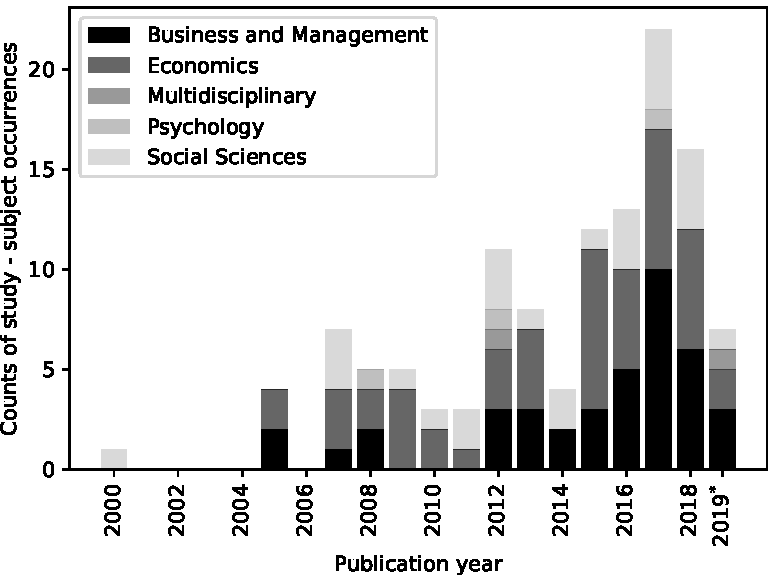
\includegraphics[width=0.65\textwidth]{A_0}
	\label{fig:disciplinary_subjs}
	\caption*{\textit{Notes.---}Disciplinary subjects as per the Scopus
	database. $^{*}$ `2019' data concern the first quarter of the year only.}
\end{figure}


\begin{table}
	\centering
	\caption{Counts of Retrieved Studies by Journal (Alphabetical Order)}
	\resizebox{0.7\textwidth}{!}{%
	\begin{tabular}{lc}
        \toprule \toprule
        Journal                                                           & Count of Studies \\
	\midrule
	Accounting Review                                                 &      1           \\
	Accounting and Business Research                                  &      1           \\
	Accounting and Finance                                            &      1           \\
	Advances in Financial Economics                                   &      1           \\
	American Economic Journal: Applied Economics                      &      4           \\
	American Economic Journal: Economic Policy                        &      1           \\
	American Economic Review                                          &      1           \\
	American Journal of Political Science                             &      4           \\
	American Journal of Sociology                                     &      1           \\
	American Political Science Review                                 &      3           \\
	Applied Economics                                                 &      1           \\
	Applied Economics Letters                                         &      2           \\
	British Accounting Review                                         &      1           \\
	Comparative Political Studies                                     &      3           \\
	Corporate Governance: An International Review                     &      1           \\
	Corporate Ownership and Control                                   &      1           \\
	Economica                                                         &      2           \\
	Electoral Studies                                                 &      3           \\
	European Journal of Economics, Finance and Administrative Science &      1           \\
	Financial Management                                              &      2           \\
	Financial Review                                                  &      1           \\
	Gender in Management                                              &      1           \\
	Human Resource Management                                         &      1           \\
	Industrial and Corporate Change                                   &      1           \\
	Industrial and Labor Relations Review                             &      1           \\
	International Interactions                                        &      1           \\
	International Journal of Social Economics                         &      1           \\
	International Studies Quarterly                                   &      1           \\
	Journal of Accounting and Economics                               &      1           \\
	Journal of Banking and Finance                                    &      2           \\
	Journal of Business Ethics                                        &      2           \\
	Journal of Business Finance and Accounting                        &      2           \\
	Journal of Business Research                                      &      2           \\
	Journal of Business Venturing                                     &      1           \\
	Journal of Comparative Economics                                  &      1           \\
	Journal of Corporate Finance                                      &      4           \\
	Journal of Economic Behavior and Organization                     &      1           \\
	Journal of Empirical Finance                                      &      1           \\
	Journal of Finance                                                &      1           \\
	Journal of Financial Economics                                    &      2           \\
	Journal of Financial Research                                     &      1           \\
	Journal of Labor Economics                                        &      1           \\
	Journal of Management                                             &      1           \\
	Journal of Public Economics                                       &      2           \\
	Leadership Quarterly                                              &      2           \\
	Management Science                                                &      2           \\
	Political Psychology                                              &      1           \\
	Proceedings of the National Academy of Sciences                   &      1           \\
	Public Administration                                             &      1           \\
	Public Administration Review                                      &      1           \\
	Public Choice                                                     &      1           \\
	Quarterly Journal of Economics                                    &      2           \\
	Review of Economic Studies                                        &      1           \\
	Review of Financial Studies                                       &      1           \\
	School Effectiveness and School Improvement                       &      1           \\
	Science                                                           &      1           \\
	Small Business Economics                                          &      3           \\
	Social Science Quarterly                                          &      1           \\
	\bottomrule
	\end{tabular}}
	\label{tab:count_by_journal}
\end{table}

\clearpage


\section{Topic Modelling of Abstracts}\label{appendix_b}

\noindent The natural language processing pipeline behind our topic model
comprises several steps (see the Jupyter notebook attached to the submission as
supplemental material). In the first step, we use the Python library
\href{https://spacy.io/}{spaCy} to pre-process the data. Specifically, we
perform the following set of string manipulations:

\begin{itemize}
	\item tokenization---sentences invo lved in the 1,156 abstracts are
		segmented into words, numbers, punctuation;
	\item lemmatization---base form of a word are applied. For example,
		the lemma of `had' is `have';
	\item token removal---numbers and stop words (i.e., words that provide
		limited information about the meanings conveyed by a piece of
	text) are filtered-out.

\end{itemize}

In the second step, we leverage the Python library
\href{https://radimrehurek.com/gensim/}{Gensim} to create the input for the
topic model, namely the \textit{dictionary} (i.e.,
the set of unique tokens involved in the corpus of abstracts) and the
\textit{corpus} (i.e., a matrix containing the numeric transformation of each
	individual abstract in terms of the set of unique tokens included in
the dictionary).

In the third step we use
\href{http://mallet.cs.umass.edu/topics.php}{Mallet} software to
estimate a set of competing topic models, each of which retains a unique
number of topics (ranging from 10 - 29 ). We set the maximum number of
topics equal to the number of categories included in Garnder and
colleagues (2010). Considering the internal validity of the models (DiMaggio,
Nag, \& Blei, 2013) and the coherence score---a statistical metrics
that expresses the face validity of the inductively derived
topics (see Mimmo, Wallach, Talley, Leenders \& McCallum, 2011)---we
retain the model with ten topics. The pattern of
topics associated with the best fitting model is shown in Figure B1.
The left-hand side of the chart employs multidimensional scaling to
offer a low-dimensional representation of the relationships among the
eleven topics. The right-hand side of the visualization reports the set
of the thirty most salient terms involved in the topic model. The live
version of this visualization---available in html format as supplemental
materials---provides additional insights regarding the pairing structure
linking terms and topics. For example, the set of the most salient terms
changes as one moves the cursor over the bullets associated with the
topics.

Finally, we use the topic model trained with Mallet to characterize each
of the 87 studies included in the review along the various topics. This
enables us to see how natural experiment methods map onto the space of
leadership phenomena and theories (at least as represented in The
Leadership Quarterly).

\noindent \textbf{References included in the Appendix}

\begin{list}{}{\setlength\itemindent{-\leftmargin}}

\item DiMaggio, P., Nag, M., \& Blei, D. (2013). Exploiting Affinities
    between Topic Modeling and the Sociological Perspective on Culture:
    Application to Newspaper Coverage of U.S. Government Arts Funding.
    \textit{Poetics} 41(6):570–606.

\item Mimno, D., Wallach, H. M., Talley, E., Leenders, M., \& McCallum, A. (2011,
July). Optimizing semantic coherence in topic models. In \textit{Proceedings of
the conference on empirical methods in natural language processing} (pp.
262-272). Association for Computational Linguistics.

\end{list}

\begin{sidewaysfigure}[!htbp]
	\centering
	\caption{Visualization of the Topic Modelling Outcome}
	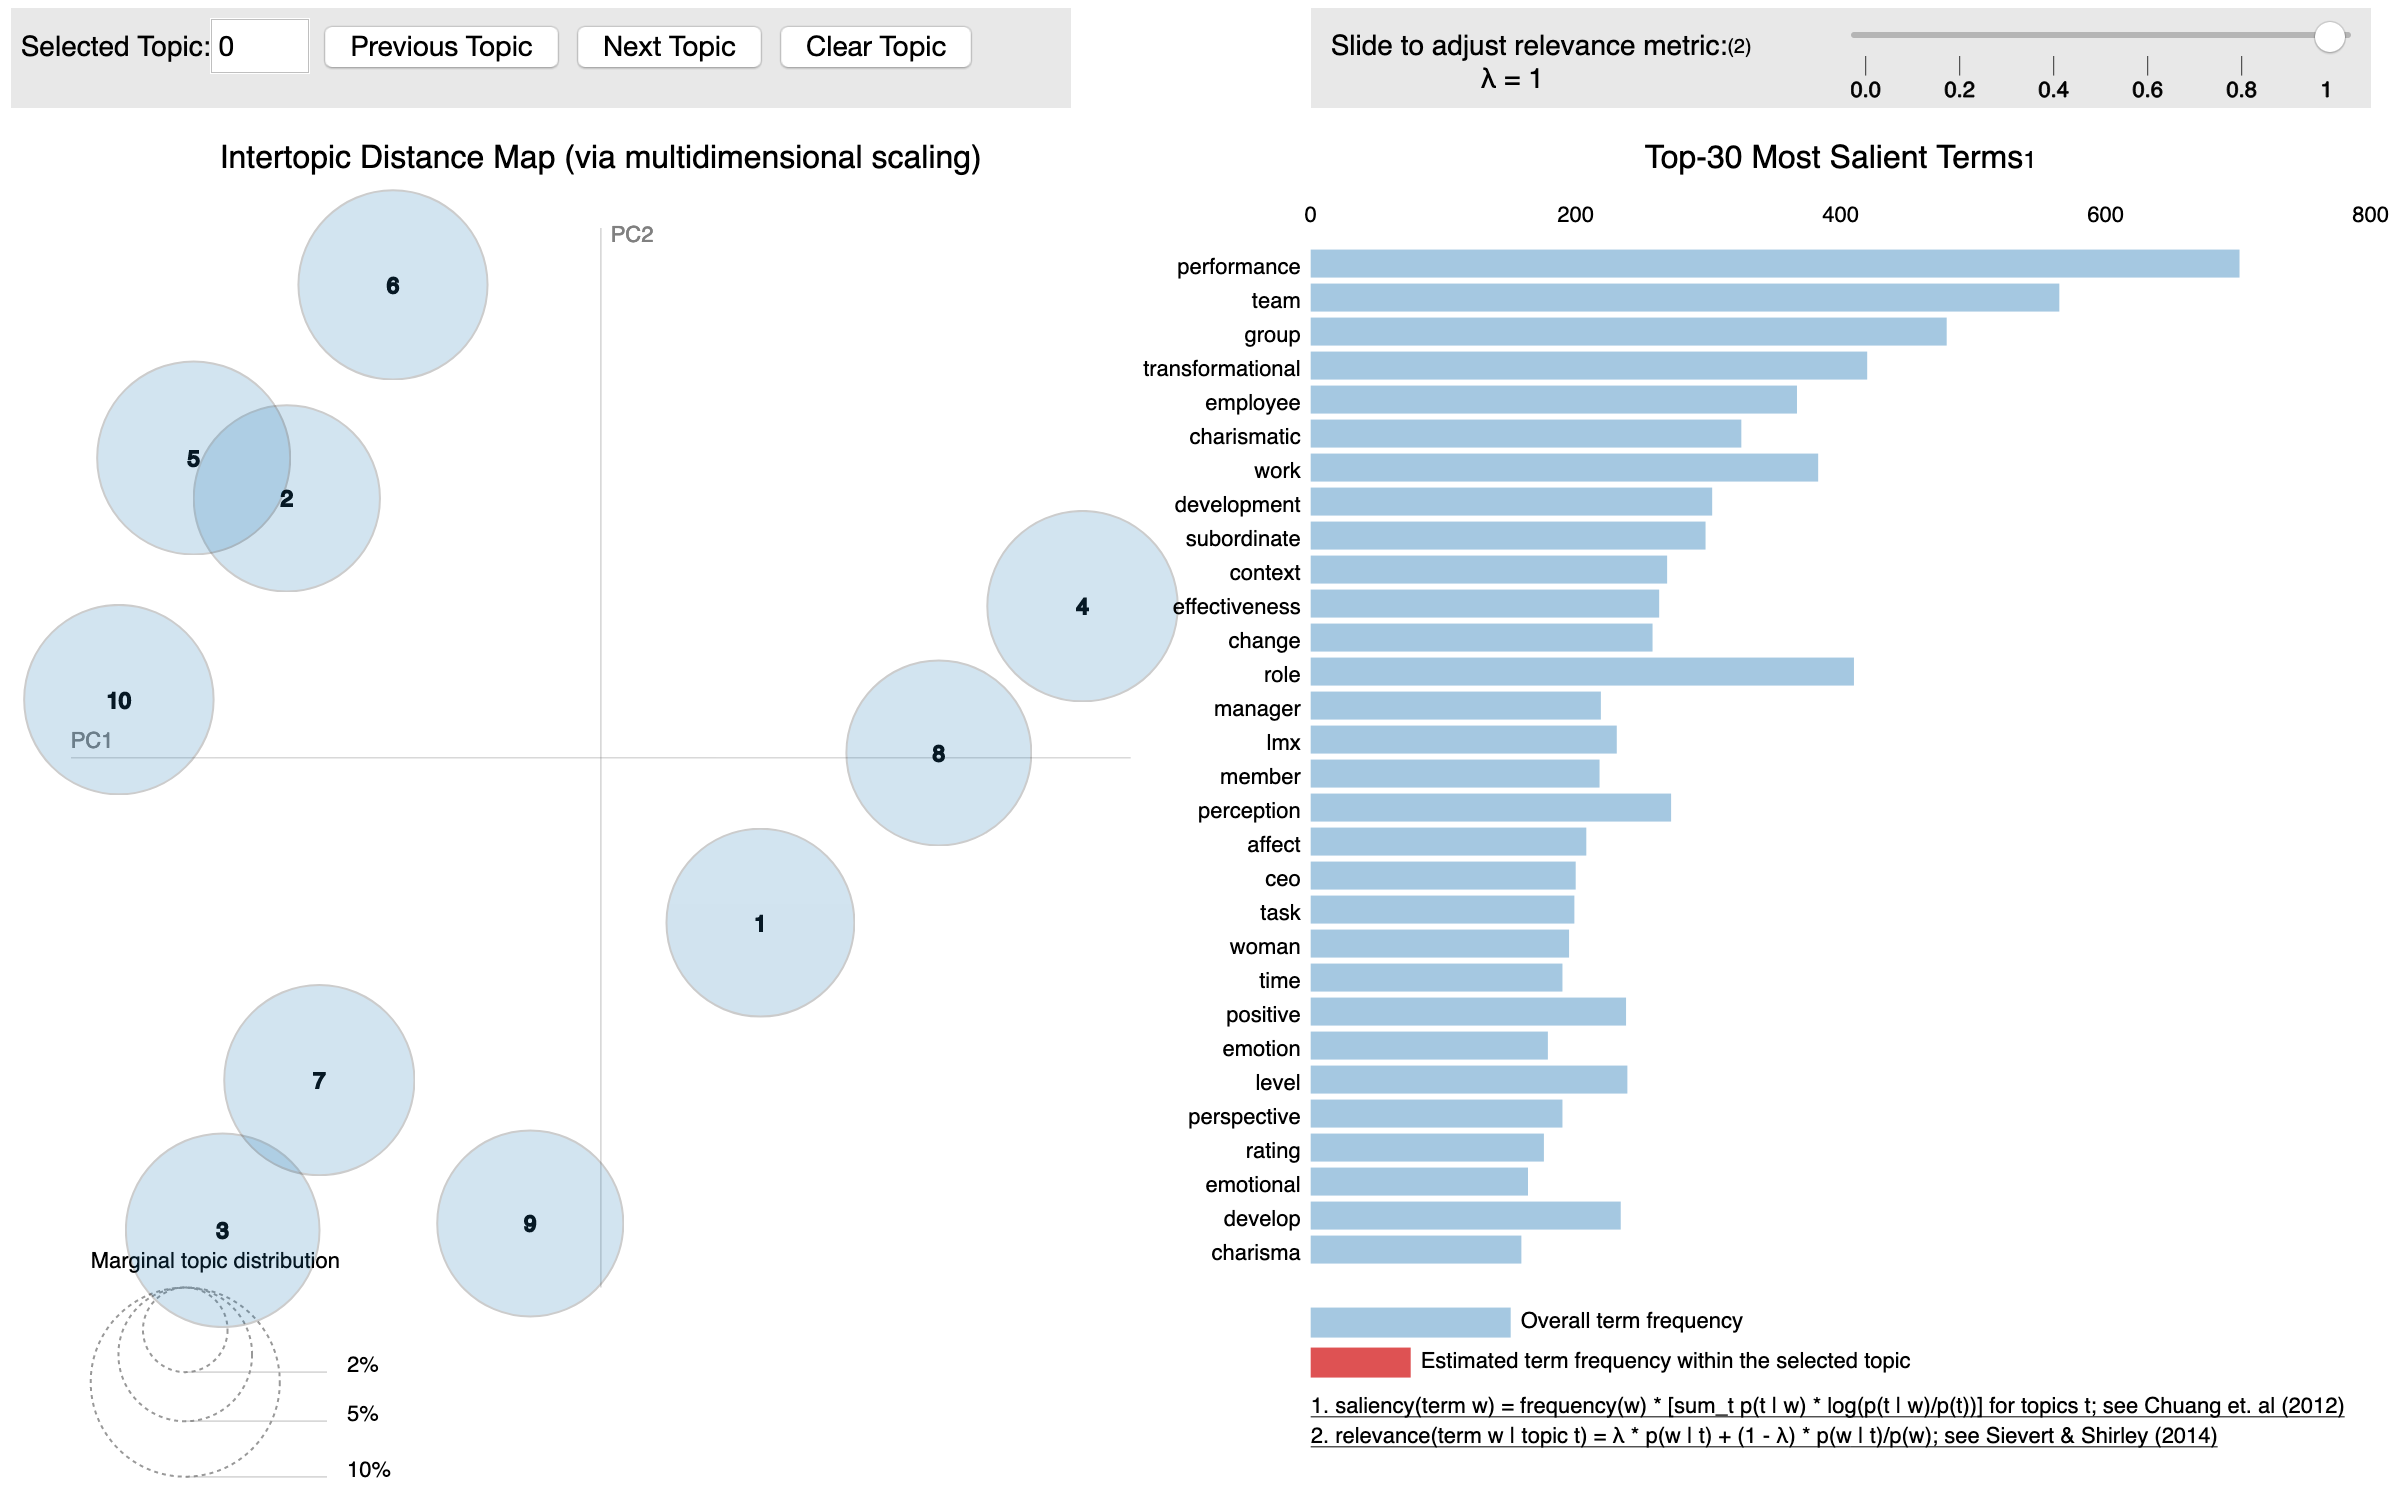
\includegraphics[width=1\textwidth]{B_1}
	\label{fig:pyldavis}
\end{sidewaysfigure}



\end{appendices}

\clearpage

%------------------------------------------------------------------------------
% document stops here
%------------------------------------------------------------------------------

\end{document}
